\documentclass[11pt]{article}

    \usepackage[breakable]{tcolorbox}
    \usepackage{parskip} % Stop auto-indenting (to mimic markdown behaviour)
    

    % Basic figure setup, for now with no caption control since it's done
    % automatically by Pandoc (which extracts ![](path) syntax from Markdown).
    \usepackage{graphicx}
    % Keep aspect ratio if custom image width or height is specified
    \setkeys{Gin}{keepaspectratio}
    % Maintain compatibility with old templates. Remove in nbconvert 6.0
    \let\Oldincludegraphics\includegraphics
    % Ensure that by default, figures have no caption (until we provide a
    % proper Figure object with a Caption API and a way to capture that
    % in the conversion process - todo).
    \usepackage{caption}
    \DeclareCaptionFormat{nocaption}{}
    \captionsetup{format=nocaption,aboveskip=0pt,belowskip=0pt}

    \usepackage{float}
    \floatplacement{figure}{H} % forces figures to be placed at the correct location
    \usepackage{xcolor} % Allow colors to be defined
    \usepackage{enumerate} % Needed for markdown enumerations to work
    \usepackage{geometry} % Used to adjust the document margins
    \usepackage{amsmath} % Equations
    \usepackage{amssymb} % Equations
    \usepackage{textcomp} % defines textquotesingle
    % Hack from http://tex.stackexchange.com/a/47451/13684:
    \AtBeginDocument{%
        \def\PYZsq{\textquotesingle}% Upright quotes in Pygmentized code
    }
    \usepackage{upquote} % Upright quotes for verbatim code
    \usepackage{eurosym} % defines \euro

    \usepackage{iftex}
    \ifPDFTeX
        \usepackage[T1]{fontenc}
        \IfFileExists{alphabeta.sty}{
              \usepackage{alphabeta}
          }{
              \usepackage[mathletters]{ucs}
              \usepackage[utf8x]{inputenc}
          }
    \else
        \usepackage{fontspec}
        \usepackage{unicode-math}
    \fi

    \usepackage{fancyvrb} % verbatim replacement that allows latex
    \usepackage{grffile} % extends the file name processing of package graphics
                         % to support a larger range
    \makeatletter % fix for old versions of grffile with XeLaTeX
    \@ifpackagelater{grffile}{2019/11/01}
    {
      % Do nothing on new versions
    }
    {
      \def\Gread@@xetex#1{%
        \IfFileExists{"\Gin@base".bb}%
        {\Gread@eps{\Gin@base.bb}}%
        {\Gread@@xetex@aux#1}%
      }
    }
    \makeatother
    \usepackage[Export]{adjustbox} % Used to constrain images to a maximum size
    \adjustboxset{max size={0.9\linewidth}{0.9\paperheight}}

    % The hyperref package gives us a pdf with properly built
    % internal navigation ('pdf bookmarks' for the table of contents,
    % internal cross-reference links, web links for URLs, etc.)
    \usepackage{hyperref}
    % The default LaTeX title has an obnoxious amount of whitespace. By default,
    % titling removes some of it. It also provides customization options.
    \usepackage{titling}
    \usepackage{longtable} % longtable support required by pandoc >1.10
    \usepackage{booktabs}  % table support for pandoc > 1.12.2
    \usepackage{array}     % table support for pandoc >= 2.11.3
    \usepackage{calc}      % table minipage width calculation for pandoc >= 2.11.1
    \usepackage[inline]{enumitem} % IRkernel/repr support (it uses the enumerate* environment)
    \usepackage[normalem]{ulem} % ulem is needed to support strikethroughs (\sout)
                                % normalem makes italics be italics, not underlines
    \usepackage{soul}      % strikethrough (\st) support for pandoc >= 3.0.0
    \usepackage{mathrsfs}
    

    
    % Colors for the hyperref package
    \definecolor{urlcolor}{rgb}{0,.145,.698}
    \definecolor{linkcolor}{rgb}{.71,0.21,0.01}
    \definecolor{citecolor}{rgb}{.12,.54,.11}

    % ANSI colors
    \definecolor{ansi-black}{HTML}{3E424D}
    \definecolor{ansi-black-intense}{HTML}{282C36}
    \definecolor{ansi-red}{HTML}{E75C58}
    \definecolor{ansi-red-intense}{HTML}{B22B31}
    \definecolor{ansi-green}{HTML}{00A250}
    \definecolor{ansi-green-intense}{HTML}{007427}
    \definecolor{ansi-yellow}{HTML}{DDB62B}
    \definecolor{ansi-yellow-intense}{HTML}{B27D12}
    \definecolor{ansi-blue}{HTML}{208FFB}
    \definecolor{ansi-blue-intense}{HTML}{0065CA}
    \definecolor{ansi-magenta}{HTML}{D160C4}
    \definecolor{ansi-magenta-intense}{HTML}{A03196}
    \definecolor{ansi-cyan}{HTML}{60C6C8}
    \definecolor{ansi-cyan-intense}{HTML}{258F8F}
    \definecolor{ansi-white}{HTML}{C5C1B4}
    \definecolor{ansi-white-intense}{HTML}{A1A6B2}
    \definecolor{ansi-default-inverse-fg}{HTML}{FFFFFF}
    \definecolor{ansi-default-inverse-bg}{HTML}{000000}

    % common color for the border for error outputs.
    \definecolor{outerrorbackground}{HTML}{FFDFDF}

    % commands and environments needed by pandoc snippets
    % extracted from the output of `pandoc -s`
    \providecommand{\tightlist}{%
      \setlength{\itemsep}{0pt}\setlength{\parskip}{0pt}}
    \DefineVerbatimEnvironment{Highlighting}{Verbatim}{commandchars=\\\{\}}
    % Add ',fontsize=\small' for more characters per line
    \newenvironment{Shaded}{}{}
    \newcommand{\KeywordTok}[1]{\textcolor[rgb]{0.00,0.44,0.13}{\textbf{{#1}}}}
    \newcommand{\DataTypeTok}[1]{\textcolor[rgb]{0.56,0.13,0.00}{{#1}}}
    \newcommand{\DecValTok}[1]{\textcolor[rgb]{0.25,0.63,0.44}{{#1}}}
    \newcommand{\BaseNTok}[1]{\textcolor[rgb]{0.25,0.63,0.44}{{#1}}}
    \newcommand{\FloatTok}[1]{\textcolor[rgb]{0.25,0.63,0.44}{{#1}}}
    \newcommand{\CharTok}[1]{\textcolor[rgb]{0.25,0.44,0.63}{{#1}}}
    \newcommand{\StringTok}[1]{\textcolor[rgb]{0.25,0.44,0.63}{{#1}}}
    \newcommand{\CommentTok}[1]{\textcolor[rgb]{0.38,0.63,0.69}{\textit{{#1}}}}
    \newcommand{\OtherTok}[1]{\textcolor[rgb]{0.00,0.44,0.13}{{#1}}}
    \newcommand{\AlertTok}[1]{\textcolor[rgb]{1.00,0.00,0.00}{\textbf{{#1}}}}
    \newcommand{\FunctionTok}[1]{\textcolor[rgb]{0.02,0.16,0.49}{{#1}}}
    \newcommand{\RegionMarkerTok}[1]{{#1}}
    \newcommand{\ErrorTok}[1]{\textcolor[rgb]{1.00,0.00,0.00}{\textbf{{#1}}}}
    \newcommand{\NormalTok}[1]{{#1}}

    % Additional commands for more recent versions of Pandoc
    \newcommand{\ConstantTok}[1]{\textcolor[rgb]{0.53,0.00,0.00}{{#1}}}
    \newcommand{\SpecialCharTok}[1]{\textcolor[rgb]{0.25,0.44,0.63}{{#1}}}
    \newcommand{\VerbatimStringTok}[1]{\textcolor[rgb]{0.25,0.44,0.63}{{#1}}}
    \newcommand{\SpecialStringTok}[1]{\textcolor[rgb]{0.73,0.40,0.53}{{#1}}}
    \newcommand{\ImportTok}[1]{{#1}}
    \newcommand{\DocumentationTok}[1]{\textcolor[rgb]{0.73,0.13,0.13}{\textit{{#1}}}}
    \newcommand{\AnnotationTok}[1]{\textcolor[rgb]{0.38,0.63,0.69}{\textbf{\textit{{#1}}}}}
    \newcommand{\CommentVarTok}[1]{\textcolor[rgb]{0.38,0.63,0.69}{\textbf{\textit{{#1}}}}}
    \newcommand{\VariableTok}[1]{\textcolor[rgb]{0.10,0.09,0.49}{{#1}}}
    \newcommand{\ControlFlowTok}[1]{\textcolor[rgb]{0.00,0.44,0.13}{\textbf{{#1}}}}
    \newcommand{\OperatorTok}[1]{\textcolor[rgb]{0.40,0.40,0.40}{{#1}}}
    \newcommand{\BuiltInTok}[1]{{#1}}
    \newcommand{\ExtensionTok}[1]{{#1}}
    \newcommand{\PreprocessorTok}[1]{\textcolor[rgb]{0.74,0.48,0.00}{{#1}}}
    \newcommand{\AttributeTok}[1]{\textcolor[rgb]{0.49,0.56,0.16}{{#1}}}
    \newcommand{\InformationTok}[1]{\textcolor[rgb]{0.38,0.63,0.69}{\textbf{\textit{{#1}}}}}
    \newcommand{\WarningTok}[1]{\textcolor[rgb]{0.38,0.63,0.69}{\textbf{\textit{{#1}}}}}
    \makeatletter
    \newsavebox\pandoc@box
    \newcommand*\pandocbounded[1]{%
      \sbox\pandoc@box{#1}%
      % scaling factors for width and height
      \Gscale@div\@tempa\textheight{\dimexpr\ht\pandoc@box+\dp\pandoc@box\relax}%
      \Gscale@div\@tempb\linewidth{\wd\pandoc@box}%
      % select the smaller of both
      \ifdim\@tempb\p@<\@tempa\p@
        \let\@tempa\@tempb
      \fi
      % scaling accordingly (\@tempa < 1)
      \ifdim\@tempa\p@<\p@
        \scalebox{\@tempa}{\usebox\pandoc@box}%
      % scaling not needed, use as it is
      \else
        \usebox{\pandoc@box}%
      \fi
    }
    \makeatother

    % Define a nice break command that doesn't care if a line doesn't already
    % exist.
    \def\br{\hspace*{\fill} \\* }
    % Math Jax compatibility definitions
    \def\gt{>}
    \def\lt{<}
    \let\Oldtex\TeX
    \let\Oldlatex\LaTeX
    \renewcommand{\TeX}{\textrm{\Oldtex}}
    \renewcommand{\LaTeX}{\textrm{\Oldlatex}}
    % Document parameters
    % Document title
    \title{LinearAlgebra}
    
    
    
    
    
    
    
% Pygments definitions
\makeatletter
\def\PY@reset{\let\PY@it=\relax \let\PY@bf=\relax%
    \let\PY@ul=\relax \let\PY@tc=\relax%
    \let\PY@bc=\relax \let\PY@ff=\relax}
\def\PY@tok#1{\csname PY@tok@#1\endcsname}
\def\PY@toks#1+{\ifx\relax#1\empty\else%
    \PY@tok{#1}\expandafter\PY@toks\fi}
\def\PY@do#1{\PY@bc{\PY@tc{\PY@ul{%
    \PY@it{\PY@bf{\PY@ff{#1}}}}}}}
\def\PY#1#2{\PY@reset\PY@toks#1+\relax+\PY@do{#2}}

\@namedef{PY@tok@w}{\def\PY@tc##1{\textcolor[rgb]{0.73,0.73,0.73}{##1}}}
\@namedef{PY@tok@c}{\let\PY@it=\textit\def\PY@tc##1{\textcolor[rgb]{0.24,0.48,0.48}{##1}}}
\@namedef{PY@tok@cp}{\def\PY@tc##1{\textcolor[rgb]{0.61,0.40,0.00}{##1}}}
\@namedef{PY@tok@k}{\let\PY@bf=\textbf\def\PY@tc##1{\textcolor[rgb]{0.00,0.50,0.00}{##1}}}
\@namedef{PY@tok@kp}{\def\PY@tc##1{\textcolor[rgb]{0.00,0.50,0.00}{##1}}}
\@namedef{PY@tok@kt}{\def\PY@tc##1{\textcolor[rgb]{0.69,0.00,0.25}{##1}}}
\@namedef{PY@tok@o}{\def\PY@tc##1{\textcolor[rgb]{0.40,0.40,0.40}{##1}}}
\@namedef{PY@tok@ow}{\let\PY@bf=\textbf\def\PY@tc##1{\textcolor[rgb]{0.67,0.13,1.00}{##1}}}
\@namedef{PY@tok@nb}{\def\PY@tc##1{\textcolor[rgb]{0.00,0.50,0.00}{##1}}}
\@namedef{PY@tok@nf}{\def\PY@tc##1{\textcolor[rgb]{0.00,0.00,1.00}{##1}}}
\@namedef{PY@tok@nc}{\let\PY@bf=\textbf\def\PY@tc##1{\textcolor[rgb]{0.00,0.00,1.00}{##1}}}
\@namedef{PY@tok@nn}{\let\PY@bf=\textbf\def\PY@tc##1{\textcolor[rgb]{0.00,0.00,1.00}{##1}}}
\@namedef{PY@tok@ne}{\let\PY@bf=\textbf\def\PY@tc##1{\textcolor[rgb]{0.80,0.25,0.22}{##1}}}
\@namedef{PY@tok@nv}{\def\PY@tc##1{\textcolor[rgb]{0.10,0.09,0.49}{##1}}}
\@namedef{PY@tok@no}{\def\PY@tc##1{\textcolor[rgb]{0.53,0.00,0.00}{##1}}}
\@namedef{PY@tok@nl}{\def\PY@tc##1{\textcolor[rgb]{0.46,0.46,0.00}{##1}}}
\@namedef{PY@tok@ni}{\let\PY@bf=\textbf\def\PY@tc##1{\textcolor[rgb]{0.44,0.44,0.44}{##1}}}
\@namedef{PY@tok@na}{\def\PY@tc##1{\textcolor[rgb]{0.41,0.47,0.13}{##1}}}
\@namedef{PY@tok@nt}{\let\PY@bf=\textbf\def\PY@tc##1{\textcolor[rgb]{0.00,0.50,0.00}{##1}}}
\@namedef{PY@tok@nd}{\def\PY@tc##1{\textcolor[rgb]{0.67,0.13,1.00}{##1}}}
\@namedef{PY@tok@s}{\def\PY@tc##1{\textcolor[rgb]{0.73,0.13,0.13}{##1}}}
\@namedef{PY@tok@sd}{\let\PY@it=\textit\def\PY@tc##1{\textcolor[rgb]{0.73,0.13,0.13}{##1}}}
\@namedef{PY@tok@si}{\let\PY@bf=\textbf\def\PY@tc##1{\textcolor[rgb]{0.64,0.35,0.47}{##1}}}
\@namedef{PY@tok@se}{\let\PY@bf=\textbf\def\PY@tc##1{\textcolor[rgb]{0.67,0.36,0.12}{##1}}}
\@namedef{PY@tok@sr}{\def\PY@tc##1{\textcolor[rgb]{0.64,0.35,0.47}{##1}}}
\@namedef{PY@tok@ss}{\def\PY@tc##1{\textcolor[rgb]{0.10,0.09,0.49}{##1}}}
\@namedef{PY@tok@sx}{\def\PY@tc##1{\textcolor[rgb]{0.00,0.50,0.00}{##1}}}
\@namedef{PY@tok@m}{\def\PY@tc##1{\textcolor[rgb]{0.40,0.40,0.40}{##1}}}
\@namedef{PY@tok@gh}{\let\PY@bf=\textbf\def\PY@tc##1{\textcolor[rgb]{0.00,0.00,0.50}{##1}}}
\@namedef{PY@tok@gu}{\let\PY@bf=\textbf\def\PY@tc##1{\textcolor[rgb]{0.50,0.00,0.50}{##1}}}
\@namedef{PY@tok@gd}{\def\PY@tc##1{\textcolor[rgb]{0.63,0.00,0.00}{##1}}}
\@namedef{PY@tok@gi}{\def\PY@tc##1{\textcolor[rgb]{0.00,0.52,0.00}{##1}}}
\@namedef{PY@tok@gr}{\def\PY@tc##1{\textcolor[rgb]{0.89,0.00,0.00}{##1}}}
\@namedef{PY@tok@ge}{\let\PY@it=\textit}
\@namedef{PY@tok@gs}{\let\PY@bf=\textbf}
\@namedef{PY@tok@ges}{\let\PY@bf=\textbf\let\PY@it=\textit}
\@namedef{PY@tok@gp}{\let\PY@bf=\textbf\def\PY@tc##1{\textcolor[rgb]{0.00,0.00,0.50}{##1}}}
\@namedef{PY@tok@go}{\def\PY@tc##1{\textcolor[rgb]{0.44,0.44,0.44}{##1}}}
\@namedef{PY@tok@gt}{\def\PY@tc##1{\textcolor[rgb]{0.00,0.27,0.87}{##1}}}
\@namedef{PY@tok@err}{\def\PY@bc##1{{\setlength{\fboxsep}{\string -\fboxrule}\fcolorbox[rgb]{1.00,0.00,0.00}{1,1,1}{\strut ##1}}}}
\@namedef{PY@tok@kc}{\let\PY@bf=\textbf\def\PY@tc##1{\textcolor[rgb]{0.00,0.50,0.00}{##1}}}
\@namedef{PY@tok@kd}{\let\PY@bf=\textbf\def\PY@tc##1{\textcolor[rgb]{0.00,0.50,0.00}{##1}}}
\@namedef{PY@tok@kn}{\let\PY@bf=\textbf\def\PY@tc##1{\textcolor[rgb]{0.00,0.50,0.00}{##1}}}
\@namedef{PY@tok@kr}{\let\PY@bf=\textbf\def\PY@tc##1{\textcolor[rgb]{0.00,0.50,0.00}{##1}}}
\@namedef{PY@tok@bp}{\def\PY@tc##1{\textcolor[rgb]{0.00,0.50,0.00}{##1}}}
\@namedef{PY@tok@fm}{\def\PY@tc##1{\textcolor[rgb]{0.00,0.00,1.00}{##1}}}
\@namedef{PY@tok@vc}{\def\PY@tc##1{\textcolor[rgb]{0.10,0.09,0.49}{##1}}}
\@namedef{PY@tok@vg}{\def\PY@tc##1{\textcolor[rgb]{0.10,0.09,0.49}{##1}}}
\@namedef{PY@tok@vi}{\def\PY@tc##1{\textcolor[rgb]{0.10,0.09,0.49}{##1}}}
\@namedef{PY@tok@vm}{\def\PY@tc##1{\textcolor[rgb]{0.10,0.09,0.49}{##1}}}
\@namedef{PY@tok@sa}{\def\PY@tc##1{\textcolor[rgb]{0.73,0.13,0.13}{##1}}}
\@namedef{PY@tok@sb}{\def\PY@tc##1{\textcolor[rgb]{0.73,0.13,0.13}{##1}}}
\@namedef{PY@tok@sc}{\def\PY@tc##1{\textcolor[rgb]{0.73,0.13,0.13}{##1}}}
\@namedef{PY@tok@dl}{\def\PY@tc##1{\textcolor[rgb]{0.73,0.13,0.13}{##1}}}
\@namedef{PY@tok@s2}{\def\PY@tc##1{\textcolor[rgb]{0.73,0.13,0.13}{##1}}}
\@namedef{PY@tok@sh}{\def\PY@tc##1{\textcolor[rgb]{0.73,0.13,0.13}{##1}}}
\@namedef{PY@tok@s1}{\def\PY@tc##1{\textcolor[rgb]{0.73,0.13,0.13}{##1}}}
\@namedef{PY@tok@mb}{\def\PY@tc##1{\textcolor[rgb]{0.40,0.40,0.40}{##1}}}
\@namedef{PY@tok@mf}{\def\PY@tc##1{\textcolor[rgb]{0.40,0.40,0.40}{##1}}}
\@namedef{PY@tok@mh}{\def\PY@tc##1{\textcolor[rgb]{0.40,0.40,0.40}{##1}}}
\@namedef{PY@tok@mi}{\def\PY@tc##1{\textcolor[rgb]{0.40,0.40,0.40}{##1}}}
\@namedef{PY@tok@il}{\def\PY@tc##1{\textcolor[rgb]{0.40,0.40,0.40}{##1}}}
\@namedef{PY@tok@mo}{\def\PY@tc##1{\textcolor[rgb]{0.40,0.40,0.40}{##1}}}
\@namedef{PY@tok@ch}{\let\PY@it=\textit\def\PY@tc##1{\textcolor[rgb]{0.24,0.48,0.48}{##1}}}
\@namedef{PY@tok@cm}{\let\PY@it=\textit\def\PY@tc##1{\textcolor[rgb]{0.24,0.48,0.48}{##1}}}
\@namedef{PY@tok@cpf}{\let\PY@it=\textit\def\PY@tc##1{\textcolor[rgb]{0.24,0.48,0.48}{##1}}}
\@namedef{PY@tok@c1}{\let\PY@it=\textit\def\PY@tc##1{\textcolor[rgb]{0.24,0.48,0.48}{##1}}}
\@namedef{PY@tok@cs}{\let\PY@it=\textit\def\PY@tc##1{\textcolor[rgb]{0.24,0.48,0.48}{##1}}}

\def\PYZbs{\char`\\}
\def\PYZus{\char`\_}
\def\PYZob{\char`\{}
\def\PYZcb{\char`\}}
\def\PYZca{\char`\^}
\def\PYZam{\char`\&}
\def\PYZlt{\char`\<}
\def\PYZgt{\char`\>}
\def\PYZsh{\char`\#}
\def\PYZpc{\char`\%}
\def\PYZdl{\char`\$}
\def\PYZhy{\char`\-}
\def\PYZsq{\char`\'}
\def\PYZdq{\char`\"}
\def\PYZti{\char`\~}
% for compatibility with earlier versions
\def\PYZat{@}
\def\PYZlb{[}
\def\PYZrb{]}
\makeatother


    % For linebreaks inside Verbatim environment from package fancyvrb.
    \makeatletter
        \newbox\Wrappedcontinuationbox
        \newbox\Wrappedvisiblespacebox
        \newcommand*\Wrappedvisiblespace {\textcolor{red}{\textvisiblespace}}
        \newcommand*\Wrappedcontinuationsymbol {\textcolor{red}{\llap{\tiny$\m@th\hookrightarrow$}}}
        \newcommand*\Wrappedcontinuationindent {3ex }
        \newcommand*\Wrappedafterbreak {\kern\Wrappedcontinuationindent\copy\Wrappedcontinuationbox}
        % Take advantage of the already applied Pygments mark-up to insert
        % potential linebreaks for TeX processing.
        %        {, <, #, %, $, ' and ": go to next line.
        %        _, }, ^, &, >, - and ~: stay at end of broken line.
        % Use of \textquotesingle for straight quote.
        \newcommand*\Wrappedbreaksatspecials {%
            \def\PYGZus{\discretionary{\char`\_}{\Wrappedafterbreak}{\char`\_}}%
            \def\PYGZob{\discretionary{}{\Wrappedafterbreak\char`\{}{\char`\{}}%
            \def\PYGZcb{\discretionary{\char`\}}{\Wrappedafterbreak}{\char`\}}}%
            \def\PYGZca{\discretionary{\char`\^}{\Wrappedafterbreak}{\char`\^}}%
            \def\PYGZam{\discretionary{\char`\&}{\Wrappedafterbreak}{\char`\&}}%
            \def\PYGZlt{\discretionary{}{\Wrappedafterbreak\char`\<}{\char`\<}}%
            \def\PYGZgt{\discretionary{\char`\>}{\Wrappedafterbreak}{\char`\>}}%
            \def\PYGZsh{\discretionary{}{\Wrappedafterbreak\char`\#}{\char`\#}}%
            \def\PYGZpc{\discretionary{}{\Wrappedafterbreak\char`\%}{\char`\%}}%
            \def\PYGZdl{\discretionary{}{\Wrappedafterbreak\char`\$}{\char`\$}}%
            \def\PYGZhy{\discretionary{\char`\-}{\Wrappedafterbreak}{\char`\-}}%
            \def\PYGZsq{\discretionary{}{\Wrappedafterbreak\textquotesingle}{\textquotesingle}}%
            \def\PYGZdq{\discretionary{}{\Wrappedafterbreak\char`\"}{\char`\"}}%
            \def\PYGZti{\discretionary{\char`\~}{\Wrappedafterbreak}{\char`\~}}%
        }
        % Some characters . , ; ? ! / are not pygmentized.
        % This macro makes them "active" and they will insert potential linebreaks
        \newcommand*\Wrappedbreaksatpunct {%
            \lccode`\~`\.\lowercase{\def~}{\discretionary{\hbox{\char`\.}}{\Wrappedafterbreak}{\hbox{\char`\.}}}%
            \lccode`\~`\,\lowercase{\def~}{\discretionary{\hbox{\char`\,}}{\Wrappedafterbreak}{\hbox{\char`\,}}}%
            \lccode`\~`\;\lowercase{\def~}{\discretionary{\hbox{\char`\;}}{\Wrappedafterbreak}{\hbox{\char`\;}}}%
            \lccode`\~`\:\lowercase{\def~}{\discretionary{\hbox{\char`\:}}{\Wrappedafterbreak}{\hbox{\char`\:}}}%
            \lccode`\~`\?\lowercase{\def~}{\discretionary{\hbox{\char`\?}}{\Wrappedafterbreak}{\hbox{\char`\?}}}%
            \lccode`\~`\!\lowercase{\def~}{\discretionary{\hbox{\char`\!}}{\Wrappedafterbreak}{\hbox{\char`\!}}}%
            \lccode`\~`\/\lowercase{\def~}{\discretionary{\hbox{\char`\/}}{\Wrappedafterbreak}{\hbox{\char`\/}}}%
            \catcode`\.\active
            \catcode`\,\active
            \catcode`\;\active
            \catcode`\:\active
            \catcode`\?\active
            \catcode`\!\active
            \catcode`\/\active
            \lccode`\~`\~
        }
    \makeatother

    \let\OriginalVerbatim=\Verbatim
    \makeatletter
    \renewcommand{\Verbatim}[1][1]{%
        %\parskip\z@skip
        \sbox\Wrappedcontinuationbox {\Wrappedcontinuationsymbol}%
        \sbox\Wrappedvisiblespacebox {\FV@SetupFont\Wrappedvisiblespace}%
        \def\FancyVerbFormatLine ##1{\hsize\linewidth
            \vtop{\raggedright\hyphenpenalty\z@\exhyphenpenalty\z@
                \doublehyphendemerits\z@\finalhyphendemerits\z@
                \strut ##1\strut}%
        }%
        % If the linebreak is at a space, the latter will be displayed as visible
        % space at end of first line, and a continuation symbol starts next line.
        % Stretch/shrink are however usually zero for typewriter font.
        \def\FV@Space {%
            \nobreak\hskip\z@ plus\fontdimen3\font minus\fontdimen4\font
            \discretionary{\copy\Wrappedvisiblespacebox}{\Wrappedafterbreak}
            {\kern\fontdimen2\font}%
        }%

        % Allow breaks at special characters using \PYG... macros.
        \Wrappedbreaksatspecials
        % Breaks at punctuation characters . , ; ? ! and / need catcode=\active
        \OriginalVerbatim[#1,codes*=\Wrappedbreaksatpunct]%
    }
    \makeatother

    % Exact colors from NB
    \definecolor{incolor}{HTML}{303F9F}
    \definecolor{outcolor}{HTML}{D84315}
    \definecolor{cellborder}{HTML}{CFCFCF}
    \definecolor{cellbackground}{HTML}{F7F7F7}

    % prompt
    \makeatletter
    \newcommand{\boxspacing}{\kern\kvtcb@left@rule\kern\kvtcb@boxsep}
    \makeatother
    \newcommand{\prompt}[4]{
        {\ttfamily\llap{{\color{#2}[#3]:\hspace{3pt}#4}}\vspace{-\baselineskip}}
    }
    

    
    % Prevent overflowing lines due to hard-to-break entities
    \sloppy
    % Setup hyperref package
    \hypersetup{
      breaklinks=true,  % so long urls are correctly broken across lines
      colorlinks=true,
      urlcolor=urlcolor,
      linkcolor=linkcolor,
      citecolor=citecolor,
      }
    % Slightly bigger margins than the latex defaults
    
    \geometry{verbose,tmargin=1in,bmargin=1in,lmargin=1in,rmargin=1in}
    
    

\begin{document}
    
    \maketitle
    
    

    
    Linear Algebra Concepts for Beginners in Machine Learning

    \textbf{Scaler:} Scaler has only value with Units ( eg: 500kg )

\textbf{Vector:} Vector has both magnitude (Value) and Direction. ( eg:
{[}1,2,3,4,5{]} or {[}{[}1{]},{[}2{]},{[}3{]},{[}4{]},{[}5{]}{]} )

\textbf{Tensor:} Tensor can be thought of as a generalization of scalars
(0-dimensional), vectors (1-dimensional), and matrices (2-dimensional)
to higher dimensions.

    \hypertarget{geomentric-representation-of-vectors}{%
\subsubsection{Geomentric Representation of
Vectors}\label{geomentric-representation-of-vectors}}

    \begin{figure}
\centering
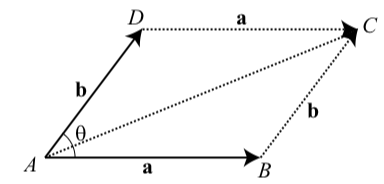
\includegraphics{LinearAlgebra_files/26f32411-e534-4edc-97bf-29252d4b9c0c.png}
\caption{GeoRepVector.png}
\end{figure}

    where,

a,b =\textgreater{} Scalers

Arrow AC is the Geomentric Representation of Vectors

    \hypertarget{vector-arithmetic}{%
\subsection{\texorpdfstring{\textbf{\emph{Vector
Arithmetic}}}{Vector Arithmetic}}\label{vector-arithmetic}}

    \hypertarget{dimensions-of-vectors}{%
\subsubsection{\texorpdfstring{\emph{1. Dimensions of
Vectors}}{1. Dimensions of Vectors}}\label{dimensions-of-vectors}}

    \begin{tcolorbox}[breakable, size=fbox, boxrule=1pt, pad at break*=1mm,colback=cellbackground, colframe=cellborder]
\prompt{In}{incolor}{1}{\boxspacing}
\begin{Verbatim}[commandchars=\\\{\}]
\PY{k+kn}{import}\PY{+w}{ }\PY{n+nn}{numpy}\PY{+w}{ }\PY{k}{as}\PY{+w}{ }\PY{n+nn}{np}
\end{Verbatim}
\end{tcolorbox}

    \begin{tcolorbox}[breakable, size=fbox, boxrule=1pt, pad at break*=1mm,colback=cellbackground, colframe=cellborder]
\prompt{In}{incolor}{2}{\boxspacing}
\begin{Verbatim}[commandchars=\\\{\}]
\PY{n}{a} \PY{o}{=} \PY{n}{np}\PY{o}{.}\PY{n}{array}\PY{p}{(}\PY{p}{[}\PY{l+m+mi}{1}\PY{p}{,}\PY{l+m+mi}{2}\PY{p}{,}\PY{l+m+mi}{3}\PY{p}{,}\PY{l+m+mi}{4}\PY{p}{,}\PY{l+m+mi}{5}\PY{p}{,}\PY{l+m+mi}{6}\PY{p}{]}\PY{p}{)}
\PY{n}{b} \PY{o}{=} \PY{n}{np}\PY{o}{.}\PY{n}{array}\PY{p}{(}\PY{p}{[}\PY{l+m+mi}{7}\PY{p}{,}\PY{l+m+mi}{8}\PY{p}{,}\PY{l+m+mi}{9}\PY{p}{,}\PY{l+m+mi}{10}\PY{p}{,}\PY{l+m+mi}{11}\PY{p}{,}\PY{l+m+mi}{12}\PY{p}{]}\PY{p}{)}
\end{Verbatim}
\end{tcolorbox}

    \begin{tcolorbox}[breakable, size=fbox, boxrule=1pt, pad at break*=1mm,colback=cellbackground, colframe=cellborder]
\prompt{In}{incolor}{3}{\boxspacing}
\begin{Verbatim}[commandchars=\\\{\}]
\PY{n+nb}{print}\PY{p}{(}\PY{n+nb}{len}\PY{p}{(}\PY{n}{a}\PY{p}{)}\PY{p}{,}\PY{n+nb}{len}\PY{p}{(}\PY{n}{b}\PY{p}{)}\PY{p}{,}\PY{n}{end}\PY{o}{=}\PY{l+s+s2}{\PYZdq{}}\PY{l+s+s2}{ }\PY{l+s+s2}{\PYZdq{}}\PY{p}{)}
\end{Verbatim}
\end{tcolorbox}

    \begin{Verbatim}[commandchars=\\\{\}]
6 6
    \end{Verbatim}

    \hypertarget{vector-addition}{%
\subsubsection{\texorpdfstring{\emph{2. Vector
Addition}}{2. Vector Addition}}\label{vector-addition}}

    \begin{tcolorbox}[breakable, size=fbox, boxrule=1pt, pad at break*=1mm,colback=cellbackground, colframe=cellborder]
\prompt{In}{incolor}{4}{\boxspacing}
\begin{Verbatim}[commandchars=\\\{\}]
\PY{n}{c} \PY{o}{=} \PY{n}{a}\PY{o}{+}\PY{n}{b}
\end{Verbatim}
\end{tcolorbox}

    \begin{tcolorbox}[breakable, size=fbox, boxrule=1pt, pad at break*=1mm,colback=cellbackground, colframe=cellborder]
\prompt{In}{incolor}{5}{\boxspacing}
\begin{Verbatim}[commandchars=\\\{\}]
\PY{n}{c}
\end{Verbatim}
\end{tcolorbox}

            \begin{tcolorbox}[breakable, size=fbox, boxrule=.5pt, pad at break*=1mm, opacityfill=0]
\prompt{Out}{outcolor}{5}{\boxspacing}
\begin{Verbatim}[commandchars=\\\{\}]
array([ 8, 10, 12, 14, 16, 18])
\end{Verbatim}
\end{tcolorbox}
        
    \textbf{Note: Different Dimensions does not support for Vector Addition}

    \begin{tcolorbox}[breakable, size=fbox, boxrule=1pt, pad at break*=1mm,colback=cellbackground, colframe=cellborder]
\prompt{In}{incolor}{6}{\boxspacing}
\begin{Verbatim}[commandchars=\\\{\}]
\PY{n}{a} \PY{o}{=} \PY{n}{np}\PY{o}{.}\PY{n}{array}\PY{p}{(}\PY{p}{[}\PY{l+m+mi}{1}\PY{p}{,}\PY{l+m+mi}{2}\PY{p}{,}\PY{l+m+mi}{3}\PY{p}{,}\PY{l+m+mi}{4}\PY{p}{]}\PY{p}{)}
\PY{n}{b} \PY{o}{=} \PY{n}{np}\PY{o}{.}\PY{n}{array}\PY{p}{(}\PY{p}{[}\PY{l+m+mi}{1}\PY{p}{,}\PY{l+m+mi}{2}\PY{p}{,}\PY{l+m+mi}{3}\PY{p}{]}\PY{p}{)}
\end{Verbatim}
\end{tcolorbox}

    \begin{tcolorbox}[breakable, size=fbox, boxrule=1pt, pad at break*=1mm,colback=cellbackground, colframe=cellborder]
\prompt{In}{incolor}{7}{\boxspacing}
\begin{Verbatim}[commandchars=\\\{\}]
\PY{n}{c} \PY{o}{=} \PY{n}{a}\PY{o}{+}\PY{n}{b}
\end{Verbatim}
\end{tcolorbox}

    \begin{Verbatim}[commandchars=\\\{\}, frame=single, framerule=2mm, rulecolor=\color{outerrorbackground}]
\textcolor{ansi-red}{---------------------------------------------------------------------------}
\textcolor{ansi-red}{ValueError}                                Traceback (most recent call last)
Cell \textcolor{ansi-green}{In[7], line 1}
\textcolor{ansi-green}{----> 1} c \def\tcRGB{\textcolor[RGB]}\expandafter\tcRGB\expandafter{\detokenize{98,98,98}}{=} a\def\tcRGB{\textcolor[RGB]}\expandafter\tcRGB\expandafter{\detokenize{98,98,98}}{+}b

\textcolor{ansi-red}{ValueError}: operands could not be broadcast together with shapes (4,) (3,) 
    \end{Verbatim}

    \hypertarget{vector-subtraction}{%
\subsubsection{\texorpdfstring{\emph{3. Vector
Subtraction}}{3. Vector Subtraction}}\label{vector-subtraction}}

    \begin{tcolorbox}[breakable, size=fbox, boxrule=1pt, pad at break*=1mm,colback=cellbackground, colframe=cellborder]
\prompt{In}{incolor}{8}{\boxspacing}
\begin{Verbatim}[commandchars=\\\{\}]
\PY{n}{a} \PY{o}{=} \PY{n}{np}\PY{o}{.}\PY{n}{array}\PY{p}{(}\PY{p}{[}\PY{l+m+mi}{5}\PY{p}{,}\PY{l+m+mi}{6}\PY{p}{,}\PY{l+m+mi}{7}\PY{p}{,}\PY{l+m+mi}{8}\PY{p}{]}\PY{p}{)}
\PY{n}{b} \PY{o}{=} \PY{n}{np}\PY{o}{.}\PY{n}{array}\PY{p}{(}\PY{p}{[}\PY{l+m+mi}{1}\PY{p}{,}\PY{l+m+mi}{2}\PY{p}{,}\PY{l+m+mi}{3}\PY{p}{,}\PY{l+m+mi}{4}\PY{p}{]}\PY{p}{)}
\end{Verbatim}
\end{tcolorbox}

    \begin{tcolorbox}[breakable, size=fbox, boxrule=1pt, pad at break*=1mm,colback=cellbackground, colframe=cellborder]
\prompt{In}{incolor}{9}{\boxspacing}
\begin{Verbatim}[commandchars=\\\{\}]
\PY{n}{c} \PY{o}{=} \PY{n}{a}\PY{o}{\PYZhy{}}\PY{n}{b}
\end{Verbatim}
\end{tcolorbox}

    \begin{tcolorbox}[breakable, size=fbox, boxrule=1pt, pad at break*=1mm,colback=cellbackground, colframe=cellborder]
\prompt{In}{incolor}{10}{\boxspacing}
\begin{Verbatim}[commandchars=\\\{\}]
\PY{n}{c}
\end{Verbatim}
\end{tcolorbox}

            \begin{tcolorbox}[breakable, size=fbox, boxrule=.5pt, pad at break*=1mm, opacityfill=0]
\prompt{Out}{outcolor}{10}{\boxspacing}
\begin{Verbatim}[commandchars=\\\{\}]
array([4, 4, 4, 4])
\end{Verbatim}
\end{tcolorbox}
        
    \textbf{Note: Different Dimensions does not support for Vector
Subtraction}

    \begin{tcolorbox}[breakable, size=fbox, boxrule=1pt, pad at break*=1mm,colback=cellbackground, colframe=cellborder]
\prompt{In}{incolor}{11}{\boxspacing}
\begin{Verbatim}[commandchars=\\\{\}]
\PY{n}{a} \PY{o}{=} \PY{n}{np}\PY{o}{.}\PY{n}{array}\PY{p}{(}\PY{p}{[}\PY{l+m+mi}{5}\PY{p}{,}\PY{l+m+mi}{6}\PY{p}{,}\PY{l+m+mi}{7}\PY{p}{,}\PY{l+m+mi}{8}\PY{p}{]}\PY{p}{)}
\PY{n}{b} \PY{o}{=} \PY{n}{np}\PY{o}{.}\PY{n}{array}\PY{p}{(}\PY{p}{[}\PY{l+m+mi}{1}\PY{p}{,}\PY{l+m+mi}{2}\PY{p}{]}\PY{p}{)}
\end{Verbatim}
\end{tcolorbox}

    \begin{tcolorbox}[breakable, size=fbox, boxrule=1pt, pad at break*=1mm,colback=cellbackground, colframe=cellborder]
\prompt{In}{incolor}{12}{\boxspacing}
\begin{Verbatim}[commandchars=\\\{\}]
\PY{n}{c} \PY{o}{=} \PY{n}{a}\PY{o}{\PYZhy{}}\PY{n}{b}
\end{Verbatim}
\end{tcolorbox}

    \begin{Verbatim}[commandchars=\\\{\}, frame=single, framerule=2mm, rulecolor=\color{outerrorbackground}]
\textcolor{ansi-red}{---------------------------------------------------------------------------}
\textcolor{ansi-red}{ValueError}                                Traceback (most recent call last)
Cell \textcolor{ansi-green}{In[12], line 1}
\textcolor{ansi-green}{----> 1} c \def\tcRGB{\textcolor[RGB]}\expandafter\tcRGB\expandafter{\detokenize{98,98,98}}{=} a\def\tcRGB{\textcolor[RGB]}\expandafter\tcRGB\expandafter{\detokenize{98,98,98}}{-}b

\textcolor{ansi-red}{ValueError}: operands could not be broadcast together with shapes (4,) (2,) 
    \end{Verbatim}

    \hypertarget{vector-multiplication}{%
\subsubsection{\texorpdfstring{4. \emph{Vector
Multiplication}}{4. Vector Multiplication}}\label{vector-multiplication}}

    \begin{tcolorbox}[breakable, size=fbox, boxrule=1pt, pad at break*=1mm,colback=cellbackground, colframe=cellborder]
\prompt{In}{incolor}{13}{\boxspacing}
\begin{Verbatim}[commandchars=\\\{\}]
\PY{n}{a} \PY{o}{=} \PY{n}{np}\PY{o}{.}\PY{n}{array}\PY{p}{(}\PY{p}{[}\PY{l+m+mi}{1}\PY{p}{,}\PY{l+m+mi}{2}\PY{p}{,}\PY{l+m+mi}{3}\PY{p}{,}\PY{l+m+mi}{4}\PY{p}{]}\PY{p}{)}
\PY{n}{b} \PY{o}{=} \PY{n}{np}\PY{o}{.}\PY{n}{array}\PY{p}{(}\PY{p}{[}\PY{l+m+mi}{1}\PY{p}{,}\PY{l+m+mi}{2}\PY{p}{,}\PY{l+m+mi}{3}\PY{p}{,}\PY{l+m+mi}{4}\PY{p}{]}\PY{p}{)}
\end{Verbatim}
\end{tcolorbox}

    \begin{tcolorbox}[breakable, size=fbox, boxrule=1pt, pad at break*=1mm,colback=cellbackground, colframe=cellborder]
\prompt{In}{incolor}{14}{\boxspacing}
\begin{Verbatim}[commandchars=\\\{\}]
\PY{n}{c} \PY{o}{=} \PY{n}{a}\PY{o}{*}\PY{n}{b}
\end{Verbatim}
\end{tcolorbox}

    \begin{tcolorbox}[breakable, size=fbox, boxrule=1pt, pad at break*=1mm,colback=cellbackground, colframe=cellborder]
\prompt{In}{incolor}{15}{\boxspacing}
\begin{Verbatim}[commandchars=\\\{\}]
\PY{n}{c}
\end{Verbatim}
\end{tcolorbox}

            \begin{tcolorbox}[breakable, size=fbox, boxrule=.5pt, pad at break*=1mm, opacityfill=0]
\prompt{Out}{outcolor}{15}{\boxspacing}
\begin{Verbatim}[commandchars=\\\{\}]
array([ 1,  4,  9, 16])
\end{Verbatim}
\end{tcolorbox}
        
    \textbf{Note: Different Dimensions doesn't support vector
multiplication}

    \begin{tcolorbox}[breakable, size=fbox, boxrule=1pt, pad at break*=1mm,colback=cellbackground, colframe=cellborder]
\prompt{In}{incolor}{16}{\boxspacing}
\begin{Verbatim}[commandchars=\\\{\}]
\PY{n}{a} \PY{o}{=} \PY{n}{np}\PY{o}{.}\PY{n}{array}\PY{p}{(}\PY{p}{[}\PY{l+m+mi}{1}\PY{p}{,}\PY{l+m+mi}{2}\PY{p}{,}\PY{l+m+mi}{3}\PY{p}{,}\PY{l+m+mi}{4}\PY{p}{]}\PY{p}{)}
\PY{n}{b} \PY{o}{=} \PY{n}{np}\PY{o}{.}\PY{n}{array}\PY{p}{(}\PY{p}{[}\PY{l+m+mi}{1}\PY{p}{,}\PY{l+m+mi}{2}\PY{p}{]}\PY{p}{)}
\end{Verbatim}
\end{tcolorbox}

    \begin{tcolorbox}[breakable, size=fbox, boxrule=1pt, pad at break*=1mm,colback=cellbackground, colframe=cellborder]
\prompt{In}{incolor}{17}{\boxspacing}
\begin{Verbatim}[commandchars=\\\{\}]
\PY{n}{c} \PY{o}{=} \PY{n}{a}\PY{o}{*}\PY{n}{b}
\end{Verbatim}
\end{tcolorbox}

    \begin{Verbatim}[commandchars=\\\{\}, frame=single, framerule=2mm, rulecolor=\color{outerrorbackground}]
\textcolor{ansi-red}{---------------------------------------------------------------------------}
\textcolor{ansi-red}{ValueError}                                Traceback (most recent call last)
Cell \textcolor{ansi-green}{In[17], line 1}
\textcolor{ansi-green}{----> 1} c \def\tcRGB{\textcolor[RGB]}\expandafter\tcRGB\expandafter{\detokenize{98,98,98}}{=} a\def\tcRGB{\textcolor[RGB]}\expandafter\tcRGB\expandafter{\detokenize{98,98,98}}{*}b

\textcolor{ansi-red}{ValueError}: operands could not be broadcast together with shapes (4,) (2,) 
    \end{Verbatim}

    \hypertarget{vector-division}{%
\subsubsection{\texorpdfstring{\emph{5. Vector
Division}}{5. Vector Division}}\label{vector-division}}

    \begin{tcolorbox}[breakable, size=fbox, boxrule=1pt, pad at break*=1mm,colback=cellbackground, colframe=cellborder]
\prompt{In}{incolor}{18}{\boxspacing}
\begin{Verbatim}[commandchars=\\\{\}]
\PY{n}{a} \PY{o}{=} \PY{n}{np}\PY{o}{.}\PY{n}{array}\PY{p}{(}\PY{p}{[}\PY{l+m+mi}{1}\PY{p}{,}\PY{l+m+mi}{2}\PY{p}{,}\PY{l+m+mi}{3}\PY{p}{,}\PY{l+m+mi}{4}\PY{p}{]}\PY{p}{)}
\PY{n}{b} \PY{o}{=} \PY{n}{np}\PY{o}{.}\PY{n}{array}\PY{p}{(}\PY{p}{[}\PY{l+m+mi}{5}\PY{p}{,}\PY{l+m+mi}{6}\PY{p}{,}\PY{l+m+mi}{7}\PY{p}{,}\PY{l+m+mi}{8}\PY{p}{]}\PY{p}{)}
\end{Verbatim}
\end{tcolorbox}

    \begin{tcolorbox}[breakable, size=fbox, boxrule=1pt, pad at break*=1mm,colback=cellbackground, colframe=cellborder]
\prompt{In}{incolor}{19}{\boxspacing}
\begin{Verbatim}[commandchars=\\\{\}]
\PY{n}{c} \PY{o}{=} \PY{n}{b}\PY{o}{/}\PY{n}{a}
\end{Verbatim}
\end{tcolorbox}

    \begin{tcolorbox}[breakable, size=fbox, boxrule=1pt, pad at break*=1mm,colback=cellbackground, colframe=cellborder]
\prompt{In}{incolor}{20}{\boxspacing}
\begin{Verbatim}[commandchars=\\\{\}]
\PY{n}{c}
\end{Verbatim}
\end{tcolorbox}

            \begin{tcolorbox}[breakable, size=fbox, boxrule=.5pt, pad at break*=1mm, opacityfill=0]
\prompt{Out}{outcolor}{20}{\boxspacing}
\begin{Verbatim}[commandchars=\\\{\}]
array([5.        , 3.        , 2.33333333, 2.        ])
\end{Verbatim}
\end{tcolorbox}
        
    \textbf{Note: Different Dimensions doesn't support Vector Division}

    \begin{tcolorbox}[breakable, size=fbox, boxrule=1pt, pad at break*=1mm,colback=cellbackground, colframe=cellborder]
\prompt{In}{incolor}{21}{\boxspacing}
\begin{Verbatim}[commandchars=\\\{\}]
\PY{n}{a} \PY{o}{=} \PY{n}{np}\PY{o}{.}\PY{n}{array}\PY{p}{(}\PY{p}{[}\PY{l+m+mi}{1}\PY{p}{,}\PY{l+m+mi}{2}\PY{p}{,}\PY{l+m+mi}{3}\PY{p}{,}\PY{l+m+mi}{4}\PY{p}{]}\PY{p}{)}
\PY{n}{b} \PY{o}{=} \PY{n}{np}\PY{o}{.}\PY{n}{array}\PY{p}{(}\PY{p}{[}\PY{l+m+mi}{1}\PY{p}{,}\PY{l+m+mi}{2}\PY{p}{]}\PY{p}{)}
\end{Verbatim}
\end{tcolorbox}

    \begin{tcolorbox}[breakable, size=fbox, boxrule=1pt, pad at break*=1mm,colback=cellbackground, colframe=cellborder]
\prompt{In}{incolor}{22}{\boxspacing}
\begin{Verbatim}[commandchars=\\\{\}]
\PY{n}{c} \PY{o}{=} \PY{n}{a}\PY{o}{/}\PY{n}{b}
\end{Verbatim}
\end{tcolorbox}

    \begin{Verbatim}[commandchars=\\\{\}, frame=single, framerule=2mm, rulecolor=\color{outerrorbackground}]
\textcolor{ansi-red}{---------------------------------------------------------------------------}
\textcolor{ansi-red}{ValueError}                                Traceback (most recent call last)
Cell \textcolor{ansi-green}{In[22], line 1}
\textcolor{ansi-green}{----> 1} c \def\tcRGB{\textcolor[RGB]}\expandafter\tcRGB\expandafter{\detokenize{98,98,98}}{=} a\def\tcRGB{\textcolor[RGB]}\expandafter\tcRGB\expandafter{\detokenize{98,98,98}}{/}b

\textcolor{ansi-red}{ValueError}: operands could not be broadcast together with shapes (4,) (2,) 
    \end{Verbatim}

    \hypertarget{vector-scaler-multiplication}{%
\subsubsection{\texorpdfstring{\emph{6. Vector Scaler
Multiplication}}{6. Vector Scaler Multiplication}}\label{vector-scaler-multiplication}}

    \begin{tcolorbox}[breakable, size=fbox, boxrule=1pt, pad at break*=1mm,colback=cellbackground, colframe=cellborder]
\prompt{In}{incolor}{23}{\boxspacing}
\begin{Verbatim}[commandchars=\\\{\}]
\PY{n}{scaler} \PY{o}{=} \PY{l+m+mi}{4}
\PY{n}{lst} \PY{o}{=} \PY{p}{[}\PY{l+m+mi}{1}\PY{p}{,}\PY{l+m+mi}{2}\PY{p}{,}\PY{l+m+mi}{3}\PY{p}{,}\PY{l+m+mi}{4}\PY{p}{,}\PY{l+m+mi}{5}\PY{p}{]}
\end{Verbatim}
\end{tcolorbox}

    \begin{tcolorbox}[breakable, size=fbox, boxrule=1pt, pad at break*=1mm,colback=cellbackground, colframe=cellborder]
\prompt{In}{incolor}{24}{\boxspacing}
\begin{Verbatim}[commandchars=\\\{\}]
\PY{n}{scaler}\PY{o}{*}\PY{n}{lst}
\end{Verbatim}
\end{tcolorbox}

            \begin{tcolorbox}[breakable, size=fbox, boxrule=.5pt, pad at break*=1mm, opacityfill=0]
\prompt{Out}{outcolor}{24}{\boxspacing}
\begin{Verbatim}[commandchars=\\\{\}]
[1, 2, 3, 4, 5, 1, 2, 3, 4, 5, 1, 2, 3, 4, 5, 1, 2, 3, 4, 5]
\end{Verbatim}
\end{tcolorbox}
        
    \begin{tcolorbox}[breakable, size=fbox, boxrule=1pt, pad at break*=1mm,colback=cellbackground, colframe=cellborder]
\prompt{In}{incolor}{25}{\boxspacing}
\begin{Verbatim}[commandchars=\\\{\}]
\PY{n}{hs} \PY{o}{=} \PY{n}{np}\PY{o}{.}\PY{n}{array}\PY{p}{(}\PY{n}{lst}\PY{p}{)}
\end{Verbatim}
\end{tcolorbox}

    \begin{tcolorbox}[breakable, size=fbox, boxrule=1pt, pad at break*=1mm,colback=cellbackground, colframe=cellborder]
\prompt{In}{incolor}{26}{\boxspacing}
\begin{Verbatim}[commandchars=\\\{\}]
\PY{n}{hs}\PY{o}{*}\PY{n}{scaler}
\end{Verbatim}
\end{tcolorbox}

            \begin{tcolorbox}[breakable, size=fbox, boxrule=.5pt, pad at break*=1mm, opacityfill=0]
\prompt{Out}{outcolor}{26}{\boxspacing}
\begin{Verbatim}[commandchars=\\\{\}]
array([ 4,  8, 12, 16, 20])
\end{Verbatim}
\end{tcolorbox}
        
    \textbf{Note: when we convert this to numpy array it follows element
multiplication}

    \hypertarget{dot-product-of-two-vectors}{%
\subsection{\texorpdfstring{\textbf{Dot Product of two
Vectors}}{Dot Product of two Vectors}}\label{dot-product-of-two-vectors}}

    \begin{figure}
\centering
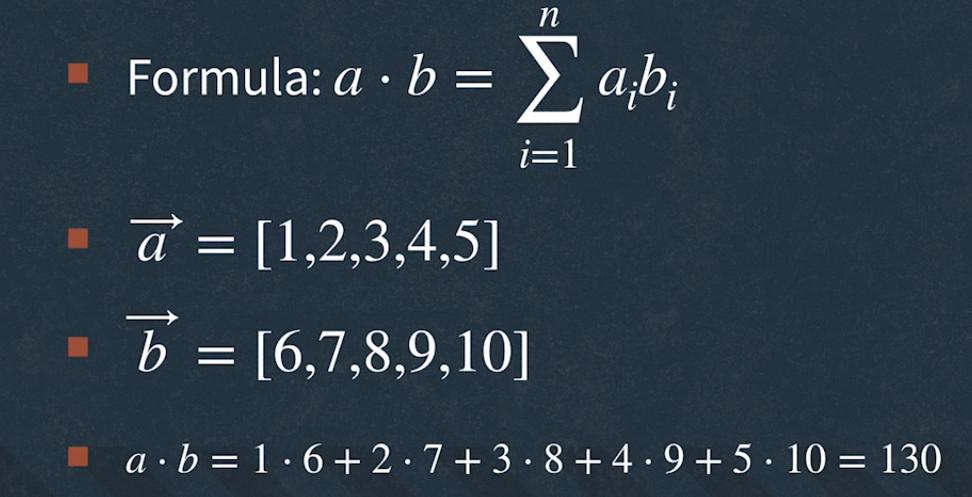
\includegraphics{Dot_product.jpg}
\caption{Dot\_product.jpg}
\end{figure}

    \begin{tcolorbox}[breakable, size=fbox, boxrule=1pt, pad at break*=1mm,colback=cellbackground, colframe=cellborder]
\prompt{In}{incolor}{27}{\boxspacing}
\begin{Verbatim}[commandchars=\\\{\}]
\PY{n}{a} \PY{o}{=} \PY{n}{np}\PY{o}{.}\PY{n}{array}\PY{p}{(}\PY{p}{[}\PY{l+m+mi}{1}\PY{p}{,}\PY{l+m+mi}{2}\PY{p}{,}\PY{l+m+mi}{3}\PY{p}{,}\PY{l+m+mi}{4}\PY{p}{]}\PY{p}{)}
\PY{n}{b} \PY{o}{=} \PY{n}{np}\PY{o}{.}\PY{n}{array}\PY{p}{(}\PY{p}{[}\PY{l+m+mi}{5}\PY{p}{,}\PY{l+m+mi}{6}\PY{p}{,}\PY{l+m+mi}{7}\PY{p}{,}\PY{l+m+mi}{8}\PY{p}{]}\PY{p}{)}
\end{Verbatim}
\end{tcolorbox}

    \begin{tcolorbox}[breakable, size=fbox, boxrule=1pt, pad at break*=1mm,colback=cellbackground, colframe=cellborder]
\prompt{In}{incolor}{28}{\boxspacing}
\begin{Verbatim}[commandchars=\\\{\}]
\PY{n+nb}{int}\PY{p}{(}\PY{n}{np}\PY{o}{.}\PY{n}{dot}\PY{p}{(}\PY{n}{a}\PY{p}{,}\PY{n}{b}\PY{p}{)}\PY{p}{)}
\end{Verbatim}
\end{tcolorbox}

            \begin{tcolorbox}[breakable, size=fbox, boxrule=.5pt, pad at break*=1mm, opacityfill=0]
\prompt{Out}{outcolor}{28}{\boxspacing}
\begin{Verbatim}[commandchars=\\\{\}]
70
\end{Verbatim}
\end{tcolorbox}
        
    \hypertarget{properties-of-dot-product}{%
\subsubsection{\texorpdfstring{\emph{Properties of Dot
product}}{Properties of Dot product}}\label{properties-of-dot-product}}

    \hypertarget{commutative-property}{%
\subsubsection{\texorpdfstring{\emph{\textbf{1. Commutative
Property}}}{1. Commutative Property}}\label{commutative-property}}

\textbf{a . b = b . a}

    \begin{tcolorbox}[breakable, size=fbox, boxrule=1pt, pad at break*=1mm,colback=cellbackground, colframe=cellborder]
\prompt{In}{incolor}{29}{\boxspacing}
\begin{Verbatim}[commandchars=\\\{\}]
\PY{n+nb}{int}\PY{p}{(}\PY{n}{np}\PY{o}{.}\PY{n}{dot}\PY{p}{(}\PY{n}{a}\PY{p}{,}\PY{n}{b}\PY{p}{)}\PY{p}{)}
\end{Verbatim}
\end{tcolorbox}

            \begin{tcolorbox}[breakable, size=fbox, boxrule=.5pt, pad at break*=1mm, opacityfill=0]
\prompt{Out}{outcolor}{29}{\boxspacing}
\begin{Verbatim}[commandchars=\\\{\}]
70
\end{Verbatim}
\end{tcolorbox}
        
    \begin{tcolorbox}[breakable, size=fbox, boxrule=1pt, pad at break*=1mm,colback=cellbackground, colframe=cellborder]
\prompt{In}{incolor}{30}{\boxspacing}
\begin{Verbatim}[commandchars=\\\{\}]
\PY{n+nb}{int}\PY{p}{(}\PY{n}{np}\PY{o}{.}\PY{n}{dot}\PY{p}{(}\PY{n}{b}\PY{p}{,}\PY{n}{a}\PY{p}{)}\PY{p}{)}
\end{Verbatim}
\end{tcolorbox}

            \begin{tcolorbox}[breakable, size=fbox, boxrule=.5pt, pad at break*=1mm, opacityfill=0]
\prompt{Out}{outcolor}{30}{\boxspacing}
\begin{Verbatim}[commandchars=\\\{\}]
70
\end{Verbatim}
\end{tcolorbox}
        
    \hypertarget{distributive-property}{%
\subsubsection{\texorpdfstring{\emph{\textbf{2. Distributive
Property}}}{2. Distributive Property}}\label{distributive-property}}

\textbf{a(b+c) = a.b + a.c}

    \begin{tcolorbox}[breakable, size=fbox, boxrule=1pt, pad at break*=1mm,colback=cellbackground, colframe=cellborder]
\prompt{In}{incolor}{31}{\boxspacing}
\begin{Verbatim}[commandchars=\\\{\}]
\PY{n}{a} \PY{o}{=} \PY{n}{np}\PY{o}{.}\PY{n}{array}\PY{p}{(}\PY{p}{[}\PY{l+m+mi}{1}\PY{p}{,}\PY{l+m+mi}{2}\PY{p}{,}\PY{l+m+mi}{3}\PY{p}{,}\PY{l+m+mi}{4}\PY{p}{]}\PY{p}{)}
\PY{n}{b} \PY{o}{=} \PY{n}{np}\PY{o}{.}\PY{n}{array}\PY{p}{(}\PY{p}{[}\PY{l+m+mi}{5}\PY{p}{,}\PY{l+m+mi}{6}\PY{p}{,}\PY{l+m+mi}{7}\PY{p}{,}\PY{l+m+mi}{8}\PY{p}{]}\PY{p}{)}
\PY{n}{c} \PY{o}{=} \PY{n}{np}\PY{o}{.}\PY{n}{array}\PY{p}{(}\PY{p}{[}\PY{l+m+mi}{9}\PY{p}{,}\PY{l+m+mi}{10}\PY{p}{,}\PY{l+m+mi}{11}\PY{p}{,}\PY{l+m+mi}{12}\PY{p}{]}\PY{p}{)}
\end{Verbatim}
\end{tcolorbox}

    \begin{tcolorbox}[breakable, size=fbox, boxrule=1pt, pad at break*=1mm,colback=cellbackground, colframe=cellborder]
\prompt{In}{incolor}{32}{\boxspacing}
\begin{Verbatim}[commandchars=\\\{\}]
\PY{n}{LHS} \PY{o}{=} \PY{n+nb}{int}\PY{p}{(}\PY{n}{np}\PY{o}{.}\PY{n}{dot}\PY{p}{(}\PY{n}{a}\PY{p}{,}\PY{n}{b}\PY{o}{+}\PY{n}{c}\PY{p}{)}\PY{p}{)}
\end{Verbatim}
\end{tcolorbox}

    \begin{tcolorbox}[breakable, size=fbox, boxrule=1pt, pad at break*=1mm,colback=cellbackground, colframe=cellborder]
\prompt{In}{incolor}{33}{\boxspacing}
\begin{Verbatim}[commandchars=\\\{\}]
\PY{n}{ab} \PY{o}{=} \PY{n+nb}{int}\PY{p}{(}\PY{n}{np}\PY{o}{.}\PY{n}{dot}\PY{p}{(}\PY{n}{a}\PY{p}{,}\PY{n}{b}\PY{p}{)}\PY{p}{)}
\PY{n}{ac} \PY{o}{=} \PY{n+nb}{int}\PY{p}{(}\PY{n}{np}\PY{o}{.}\PY{n}{dot}\PY{p}{(}\PY{n}{a}\PY{p}{,}\PY{n}{c}\PY{p}{)}\PY{p}{)}
\end{Verbatim}
\end{tcolorbox}

    \begin{tcolorbox}[breakable, size=fbox, boxrule=1pt, pad at break*=1mm,colback=cellbackground, colframe=cellborder]
\prompt{In}{incolor}{34}{\boxspacing}
\begin{Verbatim}[commandchars=\\\{\}]
\PY{n}{RHS} \PY{o}{=} \PY{n}{ab} \PY{o}{+} \PY{n}{ac}
\end{Verbatim}
\end{tcolorbox}

    \begin{tcolorbox}[breakable, size=fbox, boxrule=1pt, pad at break*=1mm,colback=cellbackground, colframe=cellborder]
\prompt{In}{incolor}{35}{\boxspacing}
\begin{Verbatim}[commandchars=\\\{\}]
\PY{n+nb}{print}\PY{p}{(}\PY{n}{LHS}\PY{p}{,}\PY{n}{RHS}\PY{p}{)}
\end{Verbatim}
\end{tcolorbox}

    \begin{Verbatim}[commandchars=\\\{\}]
180 180
    \end{Verbatim}

    \hypertarget{scalar-and-vector-projection}{%
\subsection{\texorpdfstring{\textbf{Scalar and Vector
Projection}}{Scalar and Vector Projection}}\label{scalar-and-vector-projection}}

    \textbf{Scalar Projection:} The scalar projection of a vector a onto
another vector b (denoted `projba') is a measure of how much of a lies
in the direction of b, but only as a scalar value (magnitude, without
direction).

\textbf{Formula for scalar projection:} a.b / \textbar b\textbar{}

Where,

\begin{verbatim}
• a.b = dot product of 'a' and 'b' vectors.

• |b| = magnitude of 'b' vectors.
\end{verbatim}

\textbf{Vector Projection:} The vector projection of a vector a onto
another vector b is a vector that represents the component of a that
lies along the direction of b. This projection has both magnitude and
direction.

\textbf{Formula for vector projection:} ( a.b / b.b )b (or) a.b /
\textbar\textbar b\textbar\textbar{}2

Where,

• a.b = dot product of `a' and `b' vectors.

• \textbar\textbar b\textbar\textbar{}2 = square of magnitude of `b'
vectors.

    \hypertarget{magnitude-or-norm-of-vectors}{%
\subsubsection{\texorpdfstring{\textbf{Magnitude (or) norm of
vectors}}{Magnitude (or) norm of vectors}}\label{magnitude-or-norm-of-vectors}}

    Magnitude is also called as norm (or) geomentric length of vectors.
Which defines that the distance from the tail to head vectors.

It is represented as

\begin{itemize}
\tightlist
\item
  \textbar x\textbar{} - magnitude of scalars
\item
  \textbar\textbar x\textbar\textbar{} - magnitude of vectors
\end{itemize}

    \begin{tcolorbox}[breakable, size=fbox, boxrule=1pt, pad at break*=1mm,colback=cellbackground, colframe=cellborder]
\prompt{In}{incolor}{39}{\boxspacing}
\begin{Verbatim}[commandchars=\\\{\}]
\PY{k+kn}{from}\PY{+w}{ }\PY{n+nn}{numpy}\PY{+w}{ }\PY{k+kn}{import} \PY{n}{linalg} \PY{k}{as} \PY{n}{lng}
\end{Verbatim}
\end{tcolorbox}

    \begin{tcolorbox}[breakable, size=fbox, boxrule=1pt, pad at break*=1mm,colback=cellbackground, colframe=cellborder]
\prompt{In}{incolor}{50}{\boxspacing}
\begin{Verbatim}[commandchars=\\\{\}]
\PY{n}{a} \PY{o}{=} \PY{n}{np}\PY{o}{.}\PY{n}{array}\PY{p}{(}\PY{p}{[}\PY{l+m+mi}{1}\PY{p}{,}\PY{l+m+mi}{2}\PY{p}{,}\PY{l+m+mi}{3}\PY{p}{,}\PY{l+m+mi}{4}\PY{p}{,}\PY{l+m+mi}{5}\PY{p}{]}\PY{p}{)}
\PY{n}{b} \PY{o}{=} \PY{n}{np}\PY{o}{.}\PY{n}{array}\PY{p}{(}\PY{p}{[}\PY{l+m+mi}{6}\PY{p}{,}\PY{l+m+mi}{7}\PY{p}{,}\PY{l+m+mi}{8}\PY{p}{,}\PY{l+m+mi}{9}\PY{p}{,}\PY{l+m+mi}{10}\PY{p}{]}\PY{p}{)}
\end{Verbatim}
\end{tcolorbox}

    \begin{tcolorbox}[breakable, size=fbox, boxrule=1pt, pad at break*=1mm,colback=cellbackground, colframe=cellborder]
\prompt{In}{incolor}{51}{\boxspacing}
\begin{Verbatim}[commandchars=\\\{\}]
\PY{n}{norm\PYZus{}a} \PY{o}{=} \PY{n}{lng}\PY{o}{.}\PY{n}{norm}\PY{p}{(}\PY{n}{a}\PY{p}{)}
\end{Verbatim}
\end{tcolorbox}

    \begin{tcolorbox}[breakable, size=fbox, boxrule=1pt, pad at break*=1mm,colback=cellbackground, colframe=cellborder]
\prompt{In}{incolor}{57}{\boxspacing}
\begin{Verbatim}[commandchars=\\\{\}]
\PY{n}{norm\PYZus{}a}
\end{Verbatim}
\end{tcolorbox}

            \begin{tcolorbox}[breakable, size=fbox, boxrule=.5pt, pad at break*=1mm, opacityfill=0]
\prompt{Out}{outcolor}{57}{\boxspacing}
\begin{Verbatim}[commandchars=\\\{\}]
7.416198487095663
\end{Verbatim}
\end{tcolorbox}
        
    \hypertarget{scalar-projection-of-vectors}{%
\subsubsection{Scalar projection of
vectors}\label{scalar-projection-of-vectors}}

    \begin{tcolorbox}[breakable, size=fbox, boxrule=1pt, pad at break*=1mm,colback=cellbackground, colframe=cellborder]
\prompt{In}{incolor}{58}{\boxspacing}
\begin{Verbatim}[commandchars=\\\{\}]
\PY{n}{dot\PYZus{}ab} \PY{o}{=} \PY{n}{np}\PY{o}{.}\PY{n}{dot}\PY{p}{(}\PY{n}{a}\PY{p}{,}\PY{n}{b}\PY{p}{)}
\PY{n}{norm\PYZus{}b} \PY{o}{=} \PY{n}{lng}\PY{o}{.}\PY{n}{norm}\PY{p}{(}\PY{n}{b}\PY{p}{)}
\end{Verbatim}
\end{tcolorbox}

    \begin{tcolorbox}[breakable, size=fbox, boxrule=1pt, pad at break*=1mm,colback=cellbackground, colframe=cellborder]
\prompt{In}{incolor}{59}{\boxspacing}
\begin{Verbatim}[commandchars=\\\{\}]
\PY{n}{scalar\PYZus{}projection} \PY{o}{=} \PY{n}{dot\PYZus{}ab} \PY{o}{/} \PY{n}{norm\PYZus{}b}
\end{Verbatim}
\end{tcolorbox}

    \begin{tcolorbox}[breakable, size=fbox, boxrule=1pt, pad at break*=1mm,colback=cellbackground, colframe=cellborder]
\prompt{In}{incolor}{60}{\boxspacing}
\begin{Verbatim}[commandchars=\\\{\}]
\PY{n}{scalar\PYZus{}projection}
\end{Verbatim}
\end{tcolorbox}

            \begin{tcolorbox}[breakable, size=fbox, boxrule=.5pt, pad at break*=1mm, opacityfill=0]
\prompt{Out}{outcolor}{60}{\boxspacing}
\begin{Verbatim}[commandchars=\\\{\}]
7.156264473321344
\end{Verbatim}
\end{tcolorbox}
        
    \hypertarget{vector-projection-of-vectors}{%
\subsubsection{\texorpdfstring{\emph{Vector Projection of
vectors}}{Vector Projection of vectors}}\label{vector-projection-of-vectors}}

    \begin{tcolorbox}[breakable, size=fbox, boxrule=1pt, pad at break*=1mm,colback=cellbackground, colframe=cellborder]
\prompt{In}{incolor}{55}{\boxspacing}
\begin{Verbatim}[commandchars=\\\{\}]
\PY{n}{vector\PYZus{}projection} \PY{o}{=} \PY{p}{(}\PY{n}{np}\PY{o}{.}\PY{n}{dot}\PY{p}{(}\PY{n}{a}\PY{p}{,}\PY{n}{b}\PY{p}{)} \PY{o}{/} \PY{n}{np}\PY{o}{.}\PY{n}{dot}\PY{p}{(}\PY{n}{b}\PY{p}{,}\PY{n}{b}\PY{p}{)}\PY{p}{)}\PY{o}{*}\PY{n}{b}
\end{Verbatim}
\end{tcolorbox}

    \begin{tcolorbox}[breakable, size=fbox, boxrule=1pt, pad at break*=1mm,colback=cellbackground, colframe=cellborder]
\prompt{In}{incolor}{56}{\boxspacing}
\begin{Verbatim}[commandchars=\\\{\}]
\PY{n}{vector\PYZus{}projection}
\end{Verbatim}
\end{tcolorbox}

            \begin{tcolorbox}[breakable, size=fbox, boxrule=.5pt, pad at break*=1mm, opacityfill=0]
\prompt{Out}{outcolor}{56}{\boxspacing}
\begin{Verbatim}[commandchars=\\\{\}]
array([2.36363636, 2.75757576, 3.15151515, 3.54545455, 3.93939394])
\end{Verbatim}
\end{tcolorbox}
        
    \hypertarget{change-of-basis}{%
\subsection{\texorpdfstring{\textbf{Change of
basis}}{Change of basis}}\label{change-of-basis}}

    change of basis is defined as the translation of a vector given from one
basis to another
basis.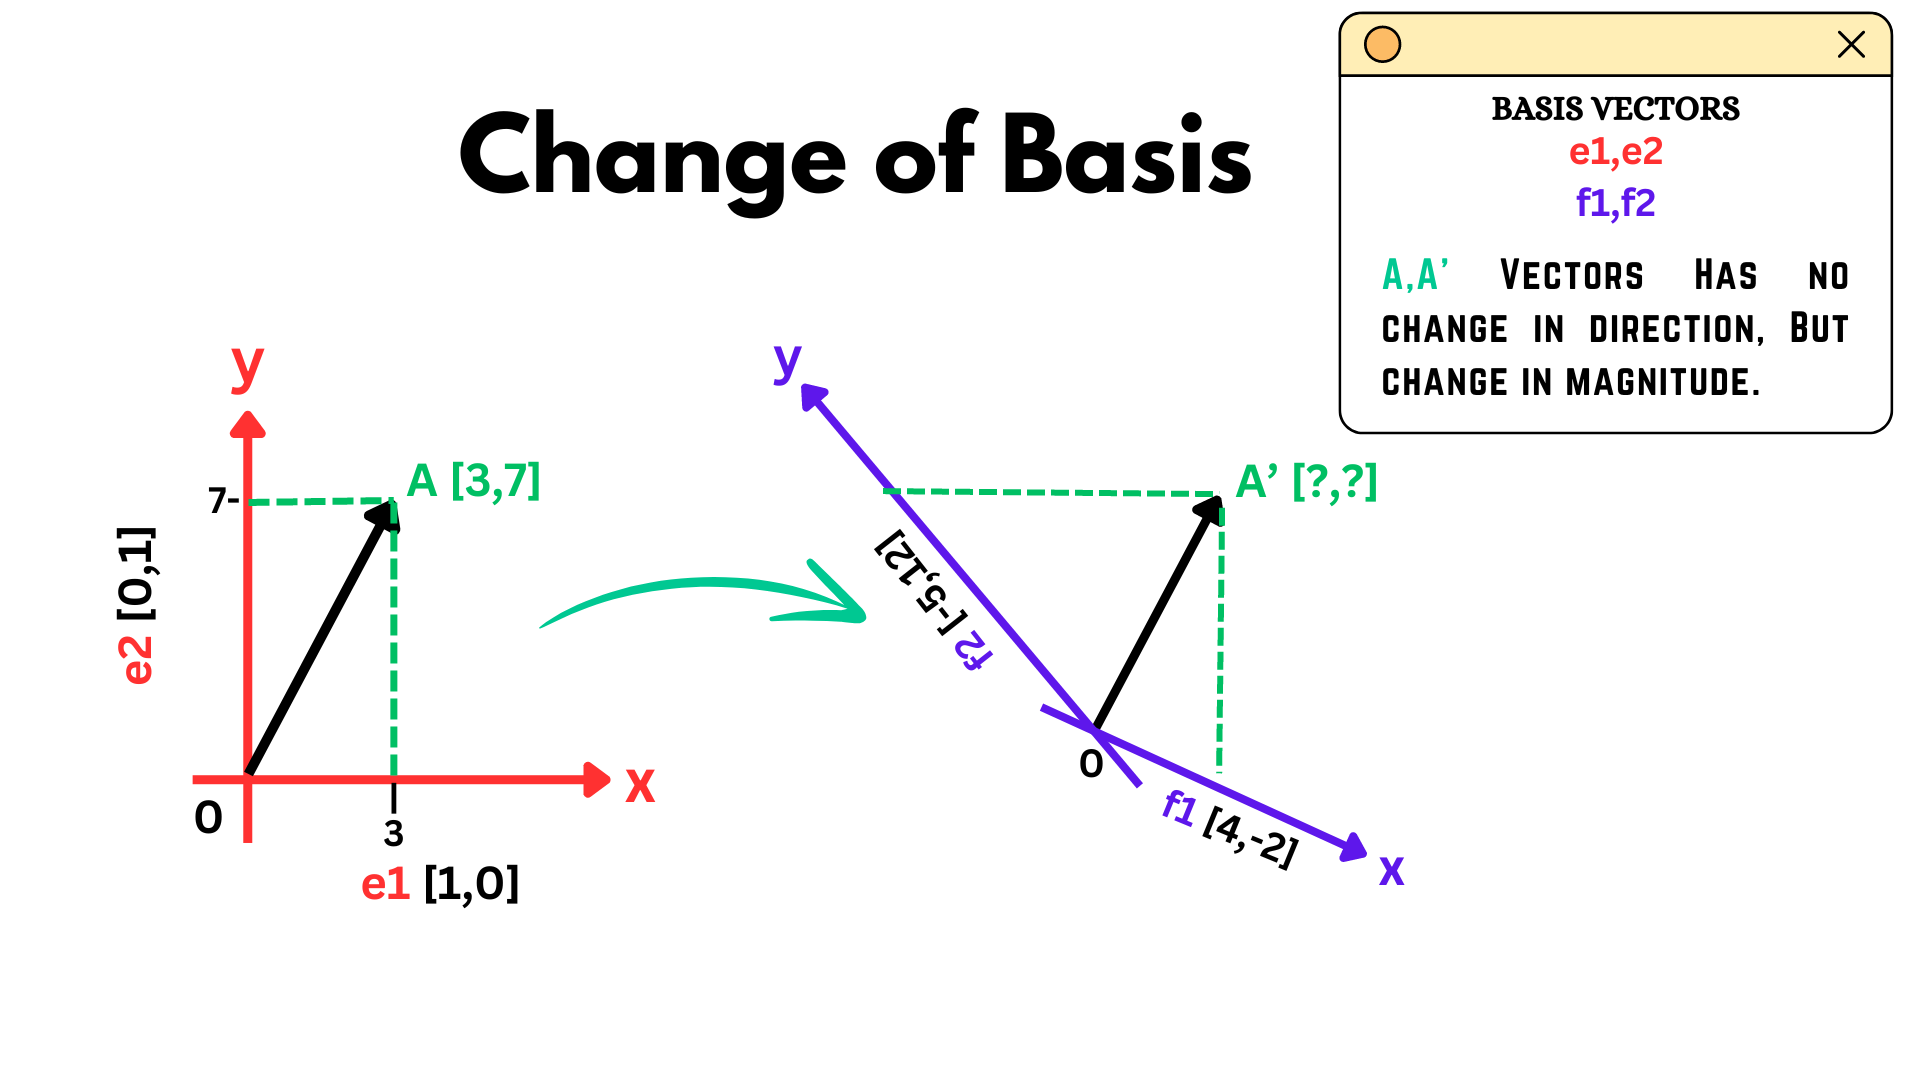
\includegraphics{LinearAlgebra_files/00aa3d79-ca83-4508-8a84-777498aa742b.png}

    Refer below pdf for calculation of basis of vectors

    \href{change_of_basis___calculation.pdf}{change of basis.pdf}

    \hypertarget{linear-combination-basis-span-linear-independence}{%
\subsection{\texorpdfstring{\textbf{Linear Combination, Basis, Span,
Linear
Independence}}{Linear Combination, Basis, Span, Linear Independence}}\label{linear-combination-basis-span-linear-independence}}

    \hypertarget{linear-combination}{%
\subsubsection{1. Linear Combination}\label{linear-combination}}

\textbf{Definition:} A linear combination of vectors
\(v_1, v_2, \ldots, v_n\) is an expression of the form
\[ s_1 v_1 + s_2 v_2 + \ldots + s_n v_n \], where \(s_i\) are scalars.

\hypertarget{linear-independence}{%
\subsubsection{2. Linear Independence}\label{linear-independence}}

\textbf{Definition:} A set of vectors \(S = \{v_1, v_2, \ldots, v_k\}\)
is said to be \textbf{linearly independent} if none of the vectors
\(v_i\) can be written as a linear combination of the other vectors.
Equivalently, the only solution to the equation
\(s_1 v_1 + s_2 v_2 + \ldots + s_k v_k = 0\) is when all \(s_i = 0\). If
there exists a solution where not all \(s_i = 0\), then the vectors are
\textbf{linearly dependent}.

\hypertarget{span-of-vectors}{%
\subsubsection{3. Span of Vectors}\label{span-of-vectors}}

\textbf{Definition:} The \textbf{span} of a set of vectors
\(\{v_1, v_2, \ldots, v_k\}\) is the set of all vectors that can be
written as a linear combination of these vectors. It is denoted as
\(\text{span}\{v_1, v_2, \ldots, v_k\}\) and includes all possible
linear combinations of the given vectors.

\hypertarget{basis}{%
\subsubsection{4. Basis}\label{basis}}

\textbf{Definition:} A \textbf{basis} for a vector space V is a set of
vectors \(B = \{b_1, b_2, \ldots, b_m\}\) that satisfies two conditions:
- \textbf{Spanning:} The set B spans the vector space V, meaning any
vector in V can be written as a linear combination of the vectors in B.
- \textbf{Linear Independence:} The set B is linearly independent,
meaning none of the vectors in B can be written as a linear combination
of the others.

\hypertarget{example}{%
\subsubsection{Example}\label{example}}

Consider the vectors \(v_1 = (2, 0, 0)\), \(v_2 = (0, 1, 0)\), and
\(v_3 = (0, 0, 7)\). These vectors are linearly independent because none
can be written as a linear combination of the others, and the only
solution to \(s_1 v_1 + s_2 v_2 + s_3 v_3 = 0\) is when
\(s_1 = s_2 = s_3 = 0\). The span of these vectors is \(\mathbb{R}^3\)
because any vector in \(\mathbb{R}^3\) can be expressed as a linear
combination of these vectors. Therefore, these vectors form a basis for
\(\mathbb{R}^3\).

    \hypertarget{analogies}{%
\subsubsection{\texorpdfstring{\textbf{Analogies}}{Analogies}}\label{analogies}}

To understand the concepts of linear combinations, linear independence,
basis, and span of vectors, we can use an analogy involving a set of
building blocks or LEGO pieces.

\hypertarget{linear-combinations}{%
\subsubsection{\texorpdfstring{1. \textbf{Linear
Combinations}}{1. Linear Combinations}}\label{linear-combinations}}

\textbf{Analogy:} Imagine you have a set of LEGO pieces of different
shapes and colors. A linear combination is like constructing a new
structure by using these LEGO pieces, where each piece can be used
multiple times and scaled (in this case, by using multiples of the same
piece). For example, if you have two types of LEGO pieces, you can build
a new structure by using 3 of the first type and 2 of the second type.
This is similar to how vectors are combined:
\[3\vec{v}_1 + 2\vec{v}_2\].

\hypertarget{linear-independence}{%
\subsubsection{\texorpdfstring{2. \textbf{Linear
Independence}}{2. Linear Independence}}\label{linear-independence}}

\textbf{Analogy:} Now, consider the LEGO pieces again. If you have a set
of pieces where no piece can be constructed by combining the others,
then these pieces are like linearly independent vectors. For instance,
if you have a square piece and a triangular piece, and neither can be
made by combining the other, they are linearly independent. If, however,
you could make the triangular piece by combining multiple square pieces,
then they would not be linearly independent.

\hypertarget{basis}{%
\subsubsection{\texorpdfstring{3.
\textbf{Basis}}{3. Basis}}\label{basis}}

\textbf{Analogy:} A basis is like a minimal set of LEGO pieces that can
be used to build any structure you want. If you have a set of pieces
that are linearly independent and can be combined to build any possible
structure, then this set is a basis. For example, if you have a set of
basic LEGO shapes (like squares, triangles, and circles) that cannot be
made from each other but can be combined to build any structure, these
shapes form a basis.

\hypertarget{span}{%
\subsubsection{\texorpdfstring{4. \textbf{Span}}{4. Span}}\label{span}}

\textbf{Analogy:} The span of a set of vectors is like the collection of
all possible structures you can build using your LEGO pieces. If you
have a set of LEGO pieces, the span is the set of all structures that
can be constructed by combining these pieces in any way. For instance,
if you have a set of square and triangular pieces, the span would
include all structures that can be built using these pieces, such as
houses, cars, or any other structure.

\hypertarget{summary}{%
\subsubsection{Summary}\label{summary}}

\begin{itemize}
\tightlist
\item
  \textbf{Linear Combinations:} Combining LEGO pieces to build new
  structures.
\item
  \textbf{Linear Independence:} Ensuring no piece can be made from the
  others.
\item
  \textbf{Basis:} A minimal set of pieces that can build any structure.
\item
  \textbf{Span:} The collection of all possible structures built from
  the pieces.
\end{itemize}

This analogy helps to visualize how these concepts work together in
linear algebra.

    \hypertarget{matrices}{%
\subsection{\texorpdfstring{\textbf{Matrices}}{Matrices}}\label{matrices}}

    Matrices are the collection of numbers with 2-dimensional arrays, which
has rows and columns.

    \begin{figure}
\centering
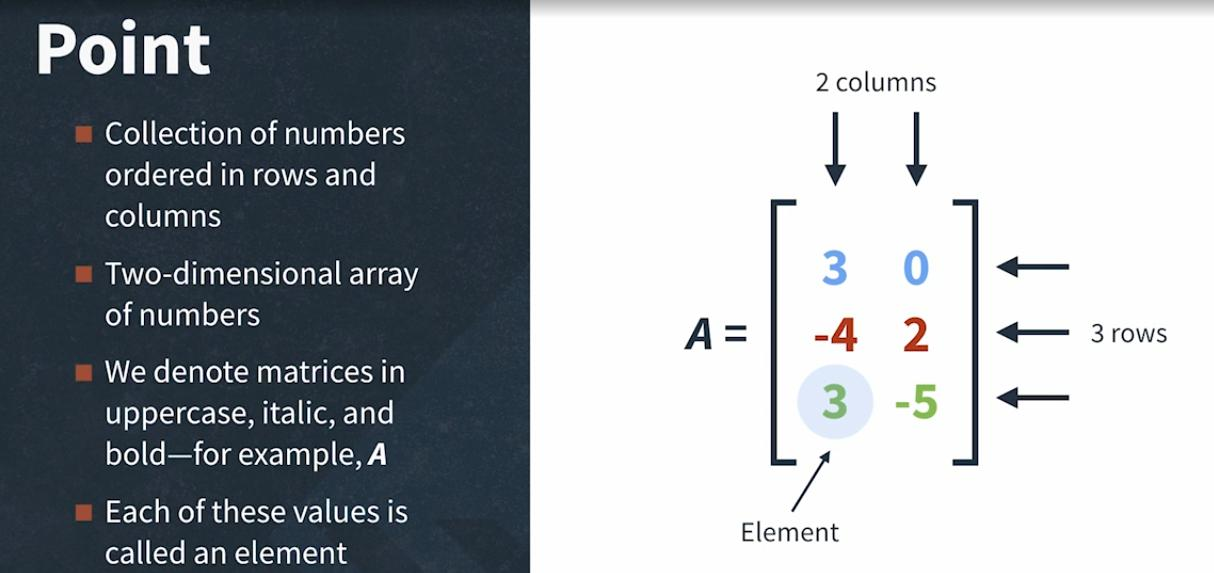
\includegraphics{LinearAlgebra_files/50637024-e1e5-4b00-980c-ef6f48fe40c6.jpg}
\caption{matrix\_intro1.jpg}
\end{figure}

    \begin{itemize}
\tightlist
\item
  Matrices element can be in any form (numbers, variables and
  expressions)
\item
  Supports all arithmetic operations.
\item
  aij represents the element of matrix `a'.
\item
  where i,j are the indexes or positions where the element is located.
\end{itemize}

    \hypertarget{seven-different-types-of-matrices}{%
\subsection{\texorpdfstring{\textbf{Seven Different types of
Matrices}}{Seven Different types of Matrices}}\label{seven-different-types-of-matrices}}

    \begin{itemize}
\tightlist
\item
  Rectangular Matrix
\item
  Square Matrix
\item
  Symmentric Matrix
\item
  Zero Matrix
\item
  Identity Matrix
\item
  Diagonal Matrix
\item
  Triangonal Matrix
\end{itemize}

    \hypertarget{rectangular-matrix}{%
\subsubsection{1) Rectangular Matrix}\label{rectangular-matrix}}

Rectangular matrix has different number of rows and columns.

\[
A = \begin{bmatrix}
12 & 14 & -5 \\
8 & -16 & 32 \\
5 & 72 & -28 \\
-35 & 83 & -92
\end{bmatrix}
\]

Here matrix A has size of 3 rows and 4 columns.

\hypertarget{square-matrix}{%
\subsubsection{2) Square Matrix}\label{square-matrix}}

Square Matrix has same number of rows and columns.

\[
A = \begin{bmatrix}
-45 & 23 \\
34 & -92 
\end{bmatrix}
\]

Here matrix A has size of 2 rows and 2 columns which are same number.

\hypertarget{symmentric-matrix}{%
\subsubsection{3) Symmentric Matrix}\label{symmentric-matrix}}

A special type of square matrix where elements are mirrored across the
diagonals.

\[
B = \begin{bmatrix}
1 & '5' & '7' \\
'5' & 2 & '9' \\
'7' & '9' & 8
\end{bmatrix}
\]

If you see the matrix `B' the numbers highlighted as quotes {[}5,7,9{]}
can be seen in the both sides of the diagonal.

\hypertarget{zero-matrix}{%
\subsubsection{4) Zero Matrix}\label{zero-matrix}}

A zero matrix is the type of matrix where all the elements in the matrix
is zero.

\[
O = \begin{bmatrix}
0 & 0 & 0 \\
0 & 0 & 0 \\
0 & 0 & 0
\end{bmatrix}
\]

\hypertarget{identity-matrix}{%
\subsubsection{5) Identity Matrix}\label{identity-matrix}}

Identity matrix is a type of square matrix where diagonal elements are
one and non-diagonal elements are zero.

\[
I = \begin{bmatrix}
1 & 0 & 0 \\
0 & 1 & 0 \\
0 & 0 & 1
\end{bmatrix}
\]

\hypertarget{diagonal-matrix}{%
\subsubsection{6) Diagonal Matrix}\label{diagonal-matrix}}

Diagonal Matrix is a type of identity matrix where diagonal elements are
represented in any numbers except zero and non diagonal matrix are zero.

\[
D = \begin{bmatrix}
13 & 0 & 0 \\
0 & 13 & 0 \\
0 & 0 & 13
\end{bmatrix}
\]

\hypertarget{triangular-matrix}{%
\subsubsection{7) Triangular Matrix}\label{triangular-matrix}}

Triangular Matrix is a square matrix where upper right or lower left of
the elements are equal to zero.

\[
T = \begin{bmatrix}
13 & 87 & 78 \\
0 & 17 & 56 \\
0 & 0 & 19
\end{bmatrix}
\]

\begin{itemize}
\tightlist
\item
  In the given matrix `T' , Right upper part above the diagonal are
  non-zeros.
\item
  In the Left lower part of the diagonal all elements are represented in
  zeros.
\end{itemize}

    \hypertarget{matrix-transformation}{%
\subsubsection{\texorpdfstring{\textbf{Matrix
Transformation}}{Matrix Transformation}}\label{matrix-transformation}}

    \textbf{Matrix transformation} is a mathematical concept where a matrix
is used to represent and perform geometric transformations on vectors.
Here's a detailed overview:

\hypertarget{what-is-matrix-transformation}{%
\subsubsection{What is Matrix
Transformation?}\label{what-is-matrix-transformation}}

A matrix transformation is a function that takes a vector in one space
and maps it to another vector in the same or a different space using
matrix multiplication. This is represented as
\[ T(\mathbf{x}) = A\mathbf{x} \], where \(A\) is the transformation
matrix, and \(\mathbf{x}\) is the input vector.

\hypertarget{types-of-matrix-transformations}{%
\subsubsection{Types of Matrix
Transformations}\label{types-of-matrix-transformations}}

Matrix transformations can be categorized into several types based on
the geometric operations they perform:

\begin{enumerate}
\def\labelenumi{\arabic{enumi}.}
\tightlist
\item
  \textbf{Translation Matrix}:

  \begin{itemize}
  \tightlist
  \item
    Moves an object along one or more axes. For example, in 3D space, a
    translation matrix can be represented as: \[
    \begin{bmatrix}
    1 & 0 & 0 & T_x \\
    0 & 1 & 0 & T_y \\
    0 & 0 & 1 & T_z \\
    0 & 0 & 0 & 1
    \end{bmatrix}
    \cdot
    \begin{pmatrix}
    x \\ y \\ z \\ 1
    \end{pmatrix}
    =
    \begin{pmatrix}
    x + T_x \\ y + T_y \\ z + T_z \\ 1
    \end{pmatrix}
    \] .
  \end{itemize}
\item
  \textbf{Rotation Matrix}:

  \begin{itemize}
  \tightlist
  \item
    Rotates an object around a specific axis. For example, a rotation
    matrix in 2D space can be: \[
    \begin{bmatrix}
    \cos(\theta) & -\sin(\theta) \\
    \sin(\theta) & \cos(\theta)
    \end{bmatrix}
    \] .
  \end{itemize}
\item
  \textbf{Scaling Matrix}:

  \begin{itemize}
  \tightlist
  \item
    Scales an object by a factor along one or more axes. For example, a
    scaling matrix in 2D space can be: \[
    \begin{bmatrix}
    k_x & 0 \\
    0 & k_y
    \end{bmatrix}
    \] .
  \end{itemize}
\item
  \textbf{Reflection Matrix}:

  \begin{itemize}
  \tightlist
  \item
    Reflects an object across a specific axis or plane. For example, a
    reflection matrix in 2D space across the x-axis can be: \[
    \begin{bmatrix}
    1 & 0 \\
    0 & -1
    \end{bmatrix}
    \] .
  \end{itemize}
\item
  \textbf{Shear Matrix}:

  \begin{itemize}
  \tightlist
  \item
    Shears an object, changing its shape by shifting it along one axis
    in proportion to its distance from another axis. For example, a
    shear matrix in 2D space can be: \[
    \begin{bmatrix}
    1 & b \\
    0 & 1
    \end{bmatrix}
    \] .
  \end{itemize}
\item
  \textbf{Affine Transformation Matrix}:

  \begin{itemize}
  \tightlist
  \item
    Preserves lines and parallelism, often used in design software.
    Affine transformations can include combinations of translation,
    rotation, scaling, and shear.
  \end{itemize}
\item
  \textbf{Projection Matrix}:

  \begin{itemize}
  \tightlist
  \item
    Projects an object onto a line or plane. This can be used to reduce
    the dimensionality of a vector.
  \end{itemize}
\end{enumerate}

\hypertarget{composition-of-transformations}{%
\subsubsection{Composition of
Transformations}\label{composition-of-transformations}}

One of the powerful aspects of matrix transformations is the ability to
compose multiple transformations by multiplying their respective
matrices. The order of multiplication is crucial, as it determines the
sequence in which the transformations are applied.

In summary, matrix transformations provide a versatile and efficient way
to perform various geometric operations, making them essential tools in
fields such as computer graphics, engineering, and physics.

    \hypertarget{understanding-rotation-matrices}{%
\subsubsection{\texorpdfstring{\textbf{Understanding Rotation
Matrices}}{Understanding Rotation Matrices}}\label{understanding-rotation-matrices}}

    To rotate a 2D vector \[\vec{x}_1 = [4, 5]\] by 30 degrees, you can use
the rotation matrix formula. Here is the step-by-step process:

\begin{enumerate}
\def\labelenumi{\arabic{enumi}.}
\item
  \textbf{Define the Rotation Matrix:} The rotation matrix for a 2D
  rotation by an angle \(\theta\) is given by: \[
  R(\theta) = \begin{bmatrix}
  \cos \theta & -\sin \theta \\
  \sin \theta & \cos \theta
  \end{bmatrix}
  \] For a rotation of 30 degrees, we need to compute \(\cos(30^\circ)\)
  and \(\sin(30^\circ)\). These values are: \[
  \cos(30^\circ) = \frac{\sqrt{3}}{2} \approx 0.866
  \] \[
  \sin(30^\circ) = \frac{1}{2} \approx 0.5
  \] So, the rotation matrix for a 30-degree rotation is: \[
  R(30^\circ) = \begin{bmatrix}
  0.866 & -0.5 \\
  0.5 & 0.866
  \end{bmatrix}
  \]
\item
  \textbf{Apply the Rotation Matrix:} Now, multiply the vector
  \[\vec{x}_1 = [4, 5]\] by the rotation matrix: \[
  \begin{bmatrix}
  x' \\ y'
  \end{bmatrix} = R(30^\circ) \begin{bmatrix}
  4 \\ 5
  \end{bmatrix}
  \] Performing the matrix multiplication: \[
  x' = 4 \cdot 0.866 - 5 \cdot 0.5 = 3.464 - 2.5 = 0.964
  \] \[
  y' = 4 \cdot 0.5 + 5 \cdot 0.866 = 2 + 4.33 = 6.33
  \] Therefore, the rotated vector is: \[
  \vec{x}'_1 = [0.964, 6.33]
  \]
\end{enumerate}

\hypertarget{summary}{%
\subsubsection{Summary}\label{summary}}

\begin{itemize}
\tightlist
\item
  \textbf{Rotation Matrix:} \[
  R(30^\circ) = \begin{bmatrix}
  0.866 & -0.5 \\
  0.5 & 0.866
  \end{bmatrix}
  \]
\item
  \textbf{Rotated Vector:} \[
  \vec{x}'_1 = [0.964, 6.33]
  \]
\end{itemize}

This method ensures that the vector is rotated correctly by 30 degrees
in the counterclockwise direction.

    \hypertarget{linear-transformation}{%
\subsubsection{\texorpdfstring{\textbf{Linear
Transformation}}{Linear Transformation}}\label{linear-transformation}}

    \hypertarget{linear-transformation-of-vectors}{%
\subsubsection{Linear Transformation of
Vectors}\label{linear-transformation-of-vectors}}

A \textbf{linear transformation} is a function between vector spaces
that preserves the operations of vector addition and scalar
multiplication. Here is a detailed explanation:

\begin{itemize}
\tightlist
\item
  \textbf{Definition}: A linear transformation
  \(T: \mathbb{R}^n \to \mathbb{R}^m\) is a function that maps vectors
  from an \(n\)-dimensional vector space to an \(m\)-dimensional vector
  space, satisfying two key properties:

  \begin{enumerate}
  \def\labelenumi{\arabic{enumi}.}
  \tightlist
  \item
    \textbf{Additivity}:
    \(T(\vec{x} + \vec{y}) = T(\vec{x}) + T(\vec{y})\) for all vectors
    \(\vec{x}\) and \(\vec{y}\) in \(\mathbb{R}^n\).
  \item
    \textbf{Homogeneity}: \(T(k\vec{x}) = kT(\vec{x})\) for all vectors
    \(\vec{x}\) in \(\mathbb{R}^n\) and all scalars \(k\).
  \end{enumerate}
\end{itemize}

\hypertarget{types-of-linear-transformations-with-examples}{%
\subsubsection{Types of Linear Transformations with
Examples}\label{types-of-linear-transformations-with-examples}}

\begin{enumerate}
\def\labelenumi{\arabic{enumi}.}
\item
  \textbf{Matrix Transformations}:

  \begin{itemize}
  \tightlist
  \item
    These are the most common form of linear transformations, where the
    transformation is defined by matrix multiplication. For example,
    given a matrix \(A\), the transformation
    \(T: \mathbb{R}^n \to \mathbb{R}^m\) defined by
    \[T(\vec{x}) = A\vec{x}\] is a linear transformation.
  \end{itemize}

  \textbf{Example}:
  \[A = \begin{pmatrix} 1 & 2 \\ 2 & 1 \end{pmatrix}\]. Then
  \(T: \mathbb{R}^2 \to \mathbb{R}^2\) defined by
  \[T\left(\begin{pmatrix} x \\ y \end{pmatrix}\right) = A\begin{pmatrix} x \\ y \end{pmatrix} = \begin{pmatrix} x + 2y \\ 2x + y \end{pmatrix}\]
  is a linear transformation.
\item
  \textbf{Identity Transformation}:

  \begin{itemize}
  \tightlist
  \item
    This transformation maps every vector to itself. It is defined by
    \(T(\vec{x}) = \vec{x}\) for all \(\vec{x}\) in the vector space.
  \end{itemize}

  \textbf{Example}: \(T: \mathbb{R}^2 \to \mathbb{R}^2\) defined by
  \[T\left(\begin{pmatrix} x \\ y \end{pmatrix}\right) = \begin{pmatrix} x \\ y \end{pmatrix}\].
\item
  \textbf{Zero Transformation}:

  \begin{itemize}
  \tightlist
  \item
    This transformation maps every vector to the zero vector. It is
    defined by \(T(\vec{x}) = \vec{0}\) for all \(\vec{x}\) in the
    vector space.
  \end{itemize}

  \textbf{Example}: \(T: \mathbb{R}^2 \to \mathbb{R}^2\) defined by
  \[T\left(\begin{pmatrix} x \\ y \end{pmatrix}\right) = \begin{pmatrix} 0 \\ 0 \end{pmatrix}\].
\item
  \textbf{Projection Transformations}:

  \begin{itemize}
  \tightlist
  \item
    These transformations project vectors onto a subspace. For example,
    projecting a vector in \(\mathbb{R}^3\) onto the \(xy\)-plane.
  \end{itemize}

  \textbf{Example}: \(T: \mathbb{R}^3 \to \mathbb{R}^3\) defined by
  \[T\left(\begin{pmatrix} x \\ y \\ z \end{pmatrix}\right) = \begin{pmatrix} x \\ y \\ 0 \end{pmatrix}\].
\item
  \textbf{Rotation Transformations}:

  \begin{itemize}
  \tightlist
  \item
    These transformations rotate vectors around an axis. For example,
    rotating a vector in \(\mathbb{R}^2\) by an angle \(\theta\).
  \end{itemize}

  \textbf{Example}: \(T: \mathbb{R}^2 \to \mathbb{R}^2\) defined by
  \[T\left(\begin{pmatrix} x \\ y \end{pmatrix}\right) = \begin{pmatrix} \cos\theta & -\sin\theta \\ \sin\theta & \cos\theta \end{pmatrix} \begin{pmatrix} x \\ y \end{pmatrix}\].
\item
  \textbf{Scaling Transformations}:

  \begin{itemize}
  \tightlist
  \item
    These transformations scale vectors by a factor. For example,
    scaling a vector in \(\mathbb{R}^2\) by a factor \(k\).
  \end{itemize}

  \textbf{Example}: \(T: \mathbb{R}^2 \to \mathbb{R}^2\) defined by
  \[T\left(\begin{pmatrix} x \\ y \end{pmatrix}\right) = \begin{pmatrix} kx \\ ky \end{pmatrix}\].
\item
  \textbf{Inverse Transformation}

  \begin{itemize}
  \tightlist
  \item
    An \textbf{inverse transformation} is a type of linear
    transformation that reverses the effect of another linear
    transformation. For a linear transformation \$ T: V \to W \$, the
    inverse transformation \$T\^{}\{-1\}: W \to V \$satisfies:

    \begin{itemize}
    \tightlist
    \item
      \$ T\^{}\{-1\}(T(\vec{v})) = \vec{v} \$ for all \$ \vec{v} \$ in
      \$ V \$
    \item
      \$ T(T\^{}\{-1\}(\vec{w})) = \vec{w} \$ for all \$ \vec{w} \$ in
      \$ W \$
    \end{itemize}
  \end{itemize}

  For example, if \$ T: \mathbb{R}\^{}2 \to \mathbb{R}\^{}2 \$ is
  defined by \$ T(x, y) = (2x, 3y) \$, then the inverse transformation
  \$ T\^{}\{-1\} \$ would be defined by
  \[ T^{-1}(x, y) = \left(\frac{x}{2}, \frac{y}{3}\right) \].
\end{enumerate}

\hypertarget{verification-of-linearity}{%
\subsubsection{Verification of
Linearity}\label{verification-of-linearity}}

To verify that a transformation is linear, one must check that it
satisfies the two properties mentioned above: additivity and
homogeneity. Here is an example of verifying linearity for a
transformation:

\textbf{Example Verification}: Consider the transformation
\(T: \mathbb{R}^2 \to \mathbb{R}^3\) defined by
\[T\left(\begin{pmatrix} x \\ y \end{pmatrix}\right) = \begin{pmatrix} x^2 \\ 2x \\ xy \end{pmatrix}\].
To check if this is linear, we need to verify the two properties:

\begin{enumerate}
\def\labelenumi{\arabic{enumi}.}
\tightlist
\item
  \textbf{Additivity}: Let
  \(\vec{x} = \begin{pmatrix} x_1 \\ y_1 \end{pmatrix}\) and
  \(\vec{y} = \begin{pmatrix} x_2 \\ y_2 \end{pmatrix}\). Then, \[
  T(\vec{x} + \vec{y}) = T\left(\begin{pmatrix} x_1 + x_2 \\ y_1 + y_2 \end{pmatrix}\right) = \begin{pmatrix} (x_1 + x_2)^2 \\ 2(x_1 + x_2) \\ (x_1 + x_2)(y_1 + y_2) \end{pmatrix}
  \] This does not equal \(T(\vec{x}) + T(\vec{y})\), so the
  transformation is not linear.
\end{enumerate}

This example illustrates that not all transformations are linear, and
verifying linearity is crucial.

    \hypertarget{composition-of-linear-transformation}{%
\subsubsection{\texorpdfstring{\textbf{Composition of Linear
Transformation}}{Composition of Linear Transformation}}\label{composition-of-linear-transformation}}

    Composition of Linear Transformation is the combination of two are more
linear transformations which are applied to get a new linear
transformation.

\textbf{formula:} \[ A(B(\vec{v})) = A.B.\vec{v} \]

Where, - A,B are the linear transformation matrices - \(\vec{v}\) is a
vector.

It majorly used in lowering computation cost by directly applying linear
transformation matrix with vectors to perform linear operations.

    \hypertarget{solving-linear-equations-using-gaussian-elimination-method}{%
\subsection{\texorpdfstring{\textbf{Solving Linear Equations using
Gaussian Elimination
Method}}{Solving Linear Equations using Gaussian Elimination Method}}\label{solving-linear-equations-using-gaussian-elimination-method}}

    Let's consider we have 3 equations,

\[ x+y-z = -2 \] \[ 2x-y+z = 5 \] \[ -x+2y+2z = 1 \]

    In order to start with Gaussian Elimination, 1st step we have to write
the equations to augumented matrix.

\textbf{Argumented Matrix:} Augumented matrix are the matrices which are
used to convert equations to matrices by adding coefficients of
variables, coeffiecients of variables and values are separated using
`\textbar{}' vertical line.

    \[
A = \begin{bmatrix}
\begin{array}{ccc|c}
1 & 1 & -1 & -2 \\
2 & -1 & 1 & 5 \\
-1 & 2 & 2 & 1 \\
\end{array}
\end{bmatrix}
\]

    The goal is to convert above augumented matrix into \textbf{Row echoleon
Form}

    \hypertarget{row-echelon-form}{%
\subsection{\texorpdfstring{\emph{\textbf{Row Echelon
Form}}}{Row Echelon Form}}\label{row-echelon-form}}

    A matrix is in \textbf{row echelon form} if it satisfies the following
conditions:

\hypertarget{conditions-for-row-echelon-form}{%
\subsection{Conditions for Row Echelon
Form}\label{conditions-for-row-echelon-form}}

\begin{enumerate}
\def\labelenumi{\arabic{enumi}.}
\tightlist
\item
  \textbf{Zero Rows at the Bottom}:

  \begin{itemize}
  \tightlist
  \item
    All rows consisting entirely of zeros must be located at the bottom
    of the matrix.
  \end{itemize}
\item
  \textbf{Leading Entries}:

  \begin{itemize}
  \tightlist
  \item
    Each non-zero row must have a \textbf{leading entry} (also known as
    a \textbf{pivot}), which is the \textbf{left-most non-zero entry in
    that row} (or) \textbf{First non-zero element in that row.} This
    leading entry must be to the right of the leading entry in the row
    above it.
  \end{itemize}
\item
  \textbf{Entries Below Leading Entries}:

  \begin{itemize}
  \tightlist
  \item
    All entries in a column below a leading entry must be zeros. This
    implies that each leading entry is the only non-zero entry in its
    column below it.
  \end{itemize}
\end{enumerate}

\hypertarget{optional-condition-on-leading-entries}{%
\subsubsection{Optional Condition on Leading
Entries}\label{optional-condition-on-leading-entries}}

\begin{itemize}
\tightlist
\item
  Some definitions and texts may not require that the leading entry be
  1, while others do. However, this requirement is typically reserved
  for the \textbf{reduced row echelon form}. In general row echelon
  form, the leading entry can be any non-zero number.
\end{itemize}

\hypertarget{examples-and-clarifications}{%
\subsubsection{Examples and
Clarifications}\label{examples-and-clarifications}}

\begin{itemize}
\item
  Here is an example of a matrix in row echelon form: \[
  \begin{bmatrix}
  1 & 2 & -1 & 4 \\
  0 & 1 & 0 & 3 \\
  0 & 0 & 1 & 2 \\
  0 & 0 & 0 & 0
  \end{bmatrix}
  \] This matrix satisfies all the conditions: zero rows are at the
  bottom, and each leading entry is to the right of the one above it.
\item
  A matrix is not in row echelon form if it violates any of these
  conditions, such as having a non-zero row below a zero row or having
  leading entries in the same column.
\end{itemize}

By ensuring these conditions are met, a matrix can be transformed into
row echelon form using Gaussian elimination, which is particularly
useful for solving systems of linear equations.

    

    Let's come into augumented matrix \$ A \$.

Inorder to convert \$ A \$ into Row Echelon Form, we have to do some
matrix row operations.

    By applying \$ R\_3 \rightarrow R\_1 + R\_3 \$, we get

    \[
A = \begin{bmatrix}
\begin{array}{ccc|c}
1 & 1 & -1 & -2 \\
2 & -1 & 1 & 5 \\
0 & 3 & 1 & -1 \\
\end{array}
\end{bmatrix}
\]

    Apply \$ R\_2 \rightarrow -2R\_1 + R\_2 \$, we get

    \[
A = \begin{bmatrix}
\begin{array}{ccc|c}
1 & 1 & -1 & -2 \\
0 & -3 & 3 & 9 \\
0 & 3 & 1 & -1 \\
\end{array}
\end{bmatrix}
\]

    Apply \$ R\_3 -\textgreater{} R\_2 + R\_3 \$, we get

    \[
A = \begin{bmatrix}
\begin{array}{ccc|c}
1 & 1 & -1 & -2 \\
0 & -3 & 3 & 9 \\
0 & 0 & 4 & 8 \\
\end{array}
\end{bmatrix}
\]

    Now the given matrix is in row echelon form, why?

\[
A = \begin{bmatrix}
\begin{array}{ccc|c}
1 & 1 & -1 & -2 \\
0 & -3 & 3 & 9 \\
0 & 0 & 4 & 8 \\
\end{array}
\end{bmatrix}
\]

\hypertarget{explanation}{%
\subsubsection{Explanation:}\label{explanation}}

\begin{enumerate}
\def\labelenumi{\arabic{enumi}.}
\tightlist
\item
  The leading entry in the first row is 1 (in the first column).
\item
  The second row's leading entry is (-3), which is in the second column,
  to the right of the leading entry in the first row.
\item
  The third row's leading entry is 4, which is in the third column, to
  the right of the leading entry in the second row.
\item
  No zero rows, and all non-zero rows are above any potential zero rows
  (though there aren't any here).
\end{enumerate}

Thus, all the conditions for row echelon form are satisfied.

    

    Now convert above augumented Row-Echelon Form matrix \$ A \$ into System
of Equations, we get,

    \[
4z = 8 \implies z = 2
\]

\[
-3y + 3z = 9 \implies -3y + 3(2) = 9 \implies -3y + 6 = 9 \implies -3y = 3 \implies y = -1
\]

\[
x + y - z = -2 \implies x + (-1) - 2 = -2 \implies x - 3 = -2 \implies x = -2 + 3 \implies x = 1
\]

    Now, we get \[ x = 1; y = -1; z = 2 \] from the system of linear
equations using Gaussian Elimination Method.

    \hypertarget{gaussian-elimination-method-and-finding-inverse-matrix}{%
\subsubsection{\texorpdfstring{\textbf{Gaussian Elimination Method and
Finding Inverse
matrix}}{Gaussian Elimination Method and Finding Inverse matrix}}\label{gaussian-elimination-method-and-finding-inverse-matrix}}

    \begin{itemize}
\tightlist
\item
  Linear equations can be solved in a few different ways
\item
  Most commonly applied techniques are elimination method and
  subsitution method.
\item
  In linear algebra, we have a different technique using matrix
  inversion.
\item
  The concept of inversion is well known starting from real numbers.
\end{itemize}

    \begin{itemize}
\tightlist
\item
  A real number \$ A \$ has a multiplicative inverse if there exists a
  number b such that a multiplied with b equals 1.
\end{itemize}

\[ a.b = 1 \rightarrow A.B = I \]

    \begin{itemize}
\tightlist
\item
  We can generalize the concept of mulitplicative inverses to matrices.
\item
  Inverse of matrix A is denoted as \$ A\^{}\{-1\}\$.
\end{itemize}

\[
    A.A^{-1} = I
\] \[
    A.B = B.A = I
\]

    \begin{itemize}
\tightlist
\item
  A matrix B such that \$ A.B = B.A = I \$ is called the inverse of the
  matrix A.
\item
  If matrix A is invertible and we want to solve the sytem, then for any
  vector b the system has a unique solution x. \[ 
  A.x = B
  \]
\item
  We can get x by multiplying both sides of an equation of the left by
  the matrix \$ A\^{}\{-1\} \$.
\end{itemize}

From the equation; \(A.x = B\) multiply \(A^{-1}\) on both sides. We
get,

\[
A^{-1}.A.x = A^{-1}.B
\]

since \(A.A^{-1} = I\),

\[
x = A^{-1}.B
\]

    \begin{tcolorbox}[breakable, size=fbox, boxrule=1pt, pad at break*=1mm,colback=cellbackground, colframe=cellborder]
\prompt{In}{incolor}{1}{\boxspacing}
\begin{Verbatim}[commandchars=\\\{\}]
\PY{k+kn}{import}\PY{+w}{ }\PY{n+nn}{numpy}\PY{+w}{ }\PY{k}{as}\PY{+w}{ }\PY{n+nn}{np}
\end{Verbatim}
\end{tcolorbox}

    \begin{tcolorbox}[breakable, size=fbox, boxrule=1pt, pad at break*=1mm,colback=cellbackground, colframe=cellborder]
\prompt{In}{incolor}{8}{\boxspacing}
\begin{Verbatim}[commandchars=\\\{\}]
\PY{n}{A} \PY{o}{=} \PY{n}{np}\PY{o}{.}\PY{n}{array}\PY{p}{(}\PY{p}{[}\PY{p}{[}\PY{l+m+mi}{12}\PY{p}{,}\PY{l+m+mi}{32}\PY{p}{]}\PY{p}{,}\PY{p}{[}\PY{l+m+mi}{23}\PY{p}{,}\PY{l+m+mi}{64}\PY{p}{]}\PY{p}{]}\PY{p}{)}
\PY{n}{A}
\end{Verbatim}
\end{tcolorbox}

            \begin{tcolorbox}[breakable, size=fbox, boxrule=.5pt, pad at break*=1mm, opacityfill=0]
\prompt{Out}{outcolor}{8}{\boxspacing}
\begin{Verbatim}[commandchars=\\\{\}]
array([[12, 32],
       [23, 64]])
\end{Verbatim}
\end{tcolorbox}
        
    Find inverse of A. (\(A^{-1}\))

    \begin{tcolorbox}[breakable, size=fbox, boxrule=1pt, pad at break*=1mm,colback=cellbackground, colframe=cellborder]
\prompt{In}{incolor}{9}{\boxspacing}
\begin{Verbatim}[commandchars=\\\{\}]
\PY{n}{Ainv} \PY{o}{=} \PY{n}{np}\PY{o}{.}\PY{n}{linalg}\PY{o}{.}\PY{n}{inv}\PY{p}{(}\PY{n}{A}\PY{p}{)}
\end{Verbatim}
\end{tcolorbox}

    \begin{tcolorbox}[breakable, size=fbox, boxrule=1pt, pad at break*=1mm,colback=cellbackground, colframe=cellborder]
\prompt{In}{incolor}{10}{\boxspacing}
\begin{Verbatim}[commandchars=\\\{\}]
\PY{n}{Ainv}
\end{Verbatim}
\end{tcolorbox}

            \begin{tcolorbox}[breakable, size=fbox, boxrule=.5pt, pad at break*=1mm, opacityfill=0]
\prompt{Out}{outcolor}{10}{\boxspacing}
\begin{Verbatim}[commandchars=\\\{\}]
array([[ 2.     , -1.     ],
       [-0.71875,  0.375  ]])
\end{Verbatim}
\end{tcolorbox}
        
    Initialize \(\vec{b}\)

    \begin{tcolorbox}[breakable, size=fbox, boxrule=1pt, pad at break*=1mm,colback=cellbackground, colframe=cellborder]
\prompt{In}{incolor}{11}{\boxspacing}
\begin{Verbatim}[commandchars=\\\{\}]
\PY{n}{b} \PY{o}{=} \PY{n}{np}\PY{o}{.}\PY{n}{array}\PY{p}{(}\PY{p}{[}\PY{l+m+mi}{41}\PY{p}{,}\PY{l+m+mi}{20}\PY{p}{]}\PY{p}{)}
\PY{n}{b}
\end{Verbatim}
\end{tcolorbox}

            \begin{tcolorbox}[breakable, size=fbox, boxrule=.5pt, pad at break*=1mm, opacityfill=0]
\prompt{Out}{outcolor}{11}{\boxspacing}
\begin{Verbatim}[commandchars=\\\{\}]
array([41, 20])
\end{Verbatim}
\end{tcolorbox}
        
    Apply \$ x = A\^{}\{-1\}.\vec{b}\$, we get

    \begin{tcolorbox}[breakable, size=fbox, boxrule=1pt, pad at break*=1mm,colback=cellbackground, colframe=cellborder]
\prompt{In}{incolor}{12}{\boxspacing}
\begin{Verbatim}[commandchars=\\\{\}]
\PY{n}{x} \PY{o}{=} \PY{n}{np}\PY{o}{.}\PY{n}{dot}\PY{p}{(}\PY{n}{Ainv}\PY{p}{,}\PY{n}{b}\PY{p}{)}
\PY{n}{x}
\end{Verbatim}
\end{tcolorbox}

            \begin{tcolorbox}[breakable, size=fbox, boxrule=.5pt, pad at break*=1mm, opacityfill=0]
\prompt{Out}{outcolor}{12}{\boxspacing}
\begin{Verbatim}[commandchars=\\\{\}]
array([ 62.     , -21.96875])
\end{Verbatim}
\end{tcolorbox}
        
    To verify \(\vec{b}\), we can just multiply \(A\) and \(x\),

    \begin{tcolorbox}[breakable, size=fbox, boxrule=1pt, pad at break*=1mm,colback=cellbackground, colframe=cellborder]
\prompt{In}{incolor}{13}{\boxspacing}
\begin{Verbatim}[commandchars=\\\{\}]
\PY{n}{np}\PY{o}{.}\PY{n}{dot}\PY{p}{(}\PY{n}{A}\PY{p}{,}\PY{n}{x}\PY{p}{)}
\end{Verbatim}
\end{tcolorbox}

            \begin{tcolorbox}[breakable, size=fbox, boxrule=.5pt, pad at break*=1mm, opacityfill=0]
\prompt{Out}{outcolor}{13}{\boxspacing}
\begin{Verbatim}[commandchars=\\\{\}]
array([41., 20.])
\end{Verbatim}
\end{tcolorbox}
        
    \begin{itemize}
\tightlist
\item
  Now, we get System of linear equations where \(x = 62; y=-21.968\), By
  verifying \(\vec{b} = [41,20]\).
\end{itemize}

    \hypertarget{the-determinant-of-a-matrix}{%
\subsection{\texorpdfstring{\textbf{The Determinant of a
Matrix}}{The Determinant of a Matrix}}\label{the-determinant-of-a-matrix}}

    \begin{itemize}
\tightlist
\item
  It enables us to map a square matrix to a scalar.
\item
  Allows to determine if a matrix can be inverted.
\item
  A determinant for a matrix A is denoted as \(det(A)\).
\item
  In the case when \(det(A) = 0\), matrix \(A^{-1}\) cannot be computed.
\item
  In special cases matrix A is singular, meaning it containts only
  linearly dependent columns.
\item
  A determinant of \(2*2\) matrix is computed using simple formula. \[
   A = \begin{bmatrix}
   a & b \\
   c & d
   \end{bmatrix}
  \] \[det(A) = a.d - b.c\]
\end{itemize}

    \begin{tcolorbox}[breakable, size=fbox, boxrule=1pt, pad at break*=1mm,colback=cellbackground, colframe=cellborder]
\prompt{In}{incolor}{23}{\boxspacing}
\begin{Verbatim}[commandchars=\\\{\}]
\PY{n}{A} \PY{o}{=} \PY{n}{np}\PY{o}{.}\PY{n}{array}\PY{p}{(}\PY{p}{[}\PY{p}{[}\PY{l+m+mi}{5}\PY{p}{,}\PY{l+m+mi}{2}\PY{p}{]}\PY{p}{,}\PY{p}{[}\PY{l+m+mi}{3}\PY{p}{,}\PY{l+m+mi}{4}\PY{p}{]}\PY{p}{]}\PY{p}{)}
\end{Verbatim}
\end{tcolorbox}

    \begin{tcolorbox}[breakable, size=fbox, boxrule=1pt, pad at break*=1mm,colback=cellbackground, colframe=cellborder]
\prompt{In}{incolor}{24}{\boxspacing}
\begin{Verbatim}[commandchars=\\\{\}]
\PY{n}{det} \PY{o}{=} \PY{n}{np}\PY{o}{.}\PY{n}{linalg}\PY{o}{.}\PY{n}{det}\PY{p}{(}\PY{n}{A}\PY{p}{)}
\PY{n}{det}
\end{Verbatim}
\end{tcolorbox}

            \begin{tcolorbox}[breakable, size=fbox, boxrule=.5pt, pad at break*=1mm, opacityfill=0]
\prompt{Out}{outcolor}{24}{\boxspacing}
\begin{Verbatim}[commandchars=\\\{\}]
13.999999999999996
\end{Verbatim}
\end{tcolorbox}
        
    \hypertarget{standard-basis-vectors}{%
\subsubsection{Standard Basis Vectors}\label{standard-basis-vectors}}

    \begin{itemize}
\tightlist
\item
  Are orthonormal, meaning they're orthogonal to each other.
\item
  They are represented as vectors a = {[}1,0{]} and b = {[}0,1{]}.
\end{itemize}

    \hypertarget{orthogonal-matrix}{%
\subsubsection{Orthogonal Matrix}\label{orthogonal-matrix}}

    \begin{itemize}
\tightlist
\item
  Usually denoted with Q
\item
  Orthonormal vectors make up all the rows and all the columns of the
  orthogonal matrix.
\end{itemize}

    \[
     Q = \begin{bmatrix}
     a & b & .. & e \\
     f & g & .. & i \\
     j & k & .. & m
     \end{bmatrix}
     \]

    \hypertarget{transpose-matrix}{%
\subsubsection{Transpose Matrix}\label{transpose-matrix}}

\begin{itemize}
\tightlist
\item
  Is a flipped version of the orginal matrix; we just have to switch
  rows and columns.
\item
  It is denoted as \(A^t\).
\end{itemize}

    \[
     A = \begin{bmatrix}
     1 & 2 & 3 \\
     4 & 5 & 6 \\
     7 & 8 & 9
     \end{bmatrix}
\] \[ \big\downarrow \] \[
     A^t = \begin{bmatrix}
     1 & 4 & 7 \\
     2 & 5 & 8 \\
     3 & 6 & 9
     \end{bmatrix}
\]

    \begin{itemize}
\tightlist
\item
  Very important property of a transpose matrix
\end{itemize}

\[A.A^t = A^t.A = I\]

where I is the Identity matrix with \$I=

\begin{bmatrix}
     1 & 0 \\
     0 & 1
     \end{bmatrix}

\$

    \hypertarget{gram-schmidt-process}{%
\subsubsection{\texorpdfstring{\textbf{Gram-Schmidt
Process}}{Gram-Schmidt Process}}\label{gram-schmidt-process}}

    \begin{itemize}
\tightlist
\item
  Used to transform any basis to orthogonal basis.
\end{itemize}

\hypertarget{steps-to-do-gram-schmidt}{%
\subsubsection{Steps to do
Gram-Schmidt}\label{steps-to-do-gram-schmidt}}

\begin{itemize}
\tightlist
\item
  If we consider a matrix with 5x5 dimensions.
\item
  The first column will be the same column.
\item
  Take second column orthogonalize relative to first column.
\item
  Apply third column orthogonlize relative to second and first column.
\item
  Apply fourth column orthogonalize relative to 3rd,2nd and 1st column.
\item
  Apply fifth column orthogonalize relative to 4th,3rd,2nd and 1st
  column. \#\#\#
\item
  Since all the columns in the matrix are orthogonal, but it is not a
  orthogonal matrix,
\item
  for that, normalize each column in the matrix (mulitplying with
  magnitude).
\item
  Finally, we get orthogonalized matrix with all columns pairwise with
  unit length.
\end{itemize}

    

    Suppose, - B = \{u1,u2,u3\} are the basis for \$ \mathbb{R}\^{}3\$. - B'
= \{v1,v2,v3\} are the orthogonal basis for \$ \mathbb{R}\^{}3 \$.

    \hypertarget{formula-to-calculate-gram-schmidt-process}{%
\subsubsection{formula to calculate gram-schmidt
process}\label{formula-to-calculate-gram-schmidt-process}}

    \begin{itemize}
\tightlist
\item
  \$ v\_1 = u\_1 \$
\item
  \$ v\_2 = u\_2 - ( u\_2 . v\_1 / v\_1 . v\_1 ) v\_1 \$
\item
  \$ v\_3 = u\_3 - ( u\_3 . v\_1 / v\_1 . v\_1) v\_1 - (u\_3 . v\_2 /
  v\_2 . v\_2 ) v\_2\$
\end{itemize}

    Consider a matrix A,

\[
     A = \begin{bmatrix}
     1 & 1 & 1 \\
     1 & 2 & 2 \\
     1 & 1 & 0
     \end{bmatrix}
\]

plugin the values into above formula we get,

\begin{figure}
\centering
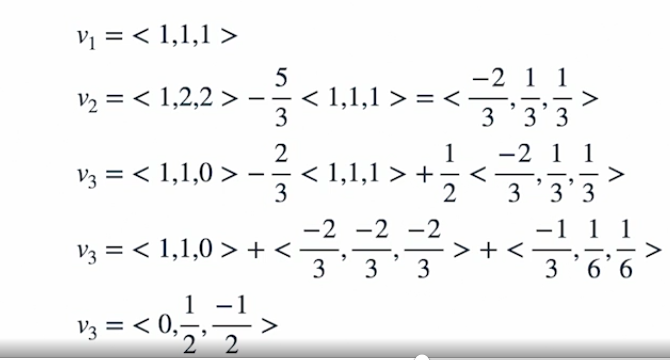
\includegraphics{LinearAlgebra_files/a89eadac-3cc0-4452-a37f-62ed6d24ee32.png}
\caption{image.png}
\end{figure}

\begin{figure}
\centering
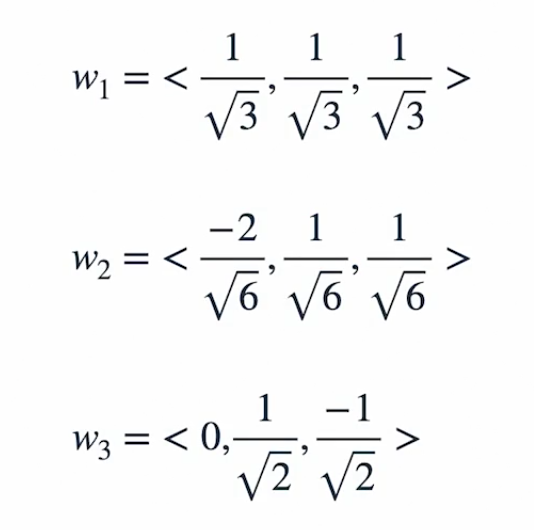
\includegraphics{LinearAlgebra_files/d5d26844-2980-4e7c-89e1-175d7cab1860.png}
\caption{image.png}
\end{figure}

    \begin{tcolorbox}[breakable, size=fbox, boxrule=1pt, pad at break*=1mm,colback=cellbackground, colframe=cellborder]
\prompt{In}{incolor}{ }{\boxspacing}
\begin{Verbatim}[commandchars=\\\{\}]

\end{Verbatim}
\end{tcolorbox}


    % Add a bibliography block to the postdoc
    
    
    
\end{document}
